\documentclass[12pt,a4paper]{article}
\usepackage[utf8]{inputenc}
\usepackage{verbatim}
\usepackage{hyperref}
\usepackage{graphicx}

%https://de.overleaf.com/learn/latex/Code_listing
\usepackage{listings}
\lstdefinestyle{mystyle}{
    backgroundcolor=\color{backcolour},
    commentstyle=\color{codegreen},
    keywordstyle=\color{magenta},
    numberstyle=\tiny\color{codegray},
    stringstyle=\color{codepurple},
    basicstyle=\ttfamily\tiny,
    breakatwhitespace=false,
    breaklines=true,
    captionpos=b,
    keepspaces=true,
    numbers=left,
    numbersep=5pt,
    showspaces=false,
    showstringspaces=false,
    showtabs=false,
    tabsize=2
}

\setlength{\headheight}{0cm}
\setlength{\headsep}{0cm}
\setlength{\topskip}{0cm}
\setlength{\topmargin}{-0.5cm}

\setlength{\parskip}{1.5ex}
\setlength{\parindent}{0cm}
\setlength{\oddsidemargin}{0cm}
\setlength{\textwidth}{16cm}
\setlength{\textheight}{25cm}

\newlength{\maximgwidth}
\setlength{\maximgwidth}{14cm}
\newcommand{\maximage}[1]{  
    \begin{center}
        \includegraphics[width=\maximgwidth]{#1} 
    \end{center}
}
\newcommand{\hint}[1]{
    \begin{center} 
        \begin{tabular}{|rp{12cm}|} \hline
            {\bf Hint}:& #1\\   \hline
        \end{tabular}
            \marginpar{\Huge !} 
    \end{center} 
}

\newcommand{\vym}{{\sc vym }}
\newcommand{\ra}{$\longrightarrow$}
\newcommand{\la}{$\longleftarrow$}
\newcommand{\ua}{$\uparrow$}
\newcommand{\da}{$\downarrow$}
\newcommand{\key}[1]{[#1]}

\newenvironment{code}[1] { \verbatim #1}{\endverbatim  }

\pagestyle{plain}
\pagenumbering{arabic}

\hypersetup{bookmarks, bookmarksopen,
  pdftitle={VYM - a tool for visual thinking },
  pdfauthor={Uwe Drechsel},    
  pdfsubject={map},
  pdfkeywords={map, tool},
  pdfpagemode={UseOutlines},                                 
  bookmarksopenlevel={1},   
  colorlinks={true},     
  linkcolor={blue},
  urlcolor={green},
  citecolor={red}}



\begin{document}
\title{
    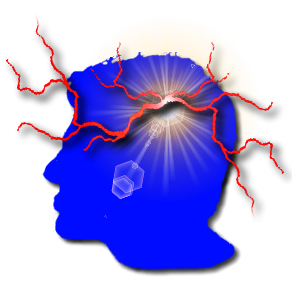
\includegraphics[width=8cm]{images/vym-logo-new.png} \\ 
    VYM  -- View Your Mind \\ 
    {\small Version 2.9.0} \\ 
    { Usermanual }
\author{\textcopyright Uwe Drechsel  }
}


\maketitle

\newpage

\tableofcontents

\newpage

\section*{Credits}
Many people have sent me their feedback and ideas, and all of that has
helped a lot to make \vym better. Thanks to all of you!

For this manual I would like to send some special thanks to

\begin{itemize}
    \item {\em Peter Adamson} for lots of feedback and proofreading of my
          far from perfect english
    \item The team of {\em AClibre (Academia y Conocimiento Libre)}
          in Colombia for their initial translation of
          the manual to spanish:
          \begin{center}
            \begin{tabular}{|p{7cm}|p{5.5cm}|} \hline
                Encargado & Actividad \\ \hline
                \begin{itemize}
                   \item Vanessa Carolina Guti\'errez Sanchez
                   \item Erika Tatiana Luque Melo
                   \item Jeffrey Steve Borb\'on Sanabria
                   \item John Edisson Ortiz Rom\'an
                \end{itemize} &
                \begin{itemize}
                    \item Traducci\'onl
                    \item Revisi\'on y correcciones varias
                    \item Estructuraci\'on y exporte
                    \item Revisi\'on y correcciones varias
                \end{itemize}     \\ \hline
            \end{tabular}   
        \end{center}
\end{itemize}
\newpage


\section{Introduction}
\subsection{What is a \vym map?}
A \vym map (abbreviated below as {\em map}) is a tree-like structure:
\maximage{images/example1.png}
Such maps can be drawn by hand on a sheet of paper or flip chart and
help to structure your thoughts. While a tree like structure like the
illustration above can be drawn manually \vym offers much more features
to work with such maps.  \vym is not just another drawing software
application, but a tool to store and modify information in an intuitive
way. For example you can reorder parts of the map by pressing a key or
add various pieces of information like a complete email by a simple
mouse click.

Once you have finished collecting and organising your ideas, you can
easily generate a variety of outputs including for example a
presentation in Open~Office based on a {\em map}.

\hint{You find the map shown above and others by clicking
\begin{center}Help \ra Open vym examples\end{center} in the menu bar.}

\subsection{Why should I use {\em maps}? Time, Space and your Brain.}
\subsubsection*{Space}
A {\em map} can concentrate very complex content in a small space such
as a piece of paper. It helps to use both sides of your brain: the
logical side and also your creative side (e.g. by using pictures,
colours and keywords in a map, often called {\em anchors}).  It is a
technique to help organize the way you think and stimulate your
creativity: It can help you by developing, sorting and helping to
memorise your ideas. 

\subsubsection*{Time}
Because you just use keywords and drawings, it is much faster than good
old fashioned 'notes'. Your brain memorizes things by associating them
with other things -- a {\em map} makes use of those connections and
stimulates new associations. 


\subsubsection*{Your Brain}
In 1960 Prof. {\sc Roger Sperry} discovered that both hemispheres
of the human brain undertake different tasks (of course both of them
basically {\em can} do the same): 
\begin{center}
\begin{tabular}{|p{5.5cm}|p{5.5cm}|} \hline
    Left side & Right side \\ \hline
    \begin{itemize}
       \item verbal speech and writing 
       \item numbers
       \item logical thinking
       \item analysing and details
       \item science
       \item linear thinking
       \item concept of time
    \end{itemize} &
    \begin{itemize}
        \item body language
        \item visual thinking, day dreams
        \item intuition and emotion
        \item overview of things
        \item creativity
        \item art, music, dancing
        \item non-linear thinking, connecting things
        \item spatial awareness
    \end{itemize}     \\ \hline
\end{tabular}   
\end{center}
In our science oriented western society we have learned to mainly rely
on our left side of the brain, the "rational" one. In other cultures,
such as the native americans and other "old" cultures, the right side is
much more important. {\em Map} are just one way to stimulate the other
side and make use of additional resources we all have.


\subsection{Where could I use a {\em map}?}
Here are some examples, how you can use those {\em maps}
\begin{itemize}
    \item to prepare articles, papers, books, talks, \ldots
    \item to sort complex data
    \item to memorize facts, peoples names, vocabulary, \ldots
    \item to sort emails, files and bookmarks on your computer
    \item to moderate conferences
    \item to brainstorm solutions to problems
    \item to record the tasks when planning a project
\end{itemize}

\subsection{What you shouldn't do with a {\em map}...}
A {\em map} drawn by somebody shows the way that the author thinks.
There is no question of right or wrong in the way it is drawn, so there
is no way to criticise it. "It is, what it is" ({\sc F.~Lehmann}).The
tool will be of considerable use to the author and only very limited use
to anyone else. 

However, when groups share in creating a {\em map} all of the group will
benefit from its use. An example of such use is when a Tutor develops a
{\em map} with a group of students during instruction. Another group use
is when a Project leader gathers a group of specialists to help {\em
map} the tasks that will be required to deliver a project.

%\section{Tutorials}
%TODO

\subsection{Internet Ressources} 
There are a few tutorial vides on youtube:
\begin{itemize}
    \item Youtube: 
        \href{https://www.youtube.com/c/ViewYourMind}{https://www.youtube.com/c/ViewYourMind}
\end{itemize}
A good starting point to learn more about Mindmaps in general is Wikipedia:
\begin{itemize}
    \item English: 
        \href{http://en.wikipedia.org/wiki/Mind_map}{http://en.wikipedia.org/wiki/Mind\_map}
    \item German: 
        \href{http://de.wikipedia.org/wiki/Mindmap}{http://de.wikipedia.org/wiki/Mindmap}
\end{itemize}





\newpage
\section{The Concept of the \vym application}
%FIXME-3 maybe add a general introduction here...
\subsection{The Mainwindow and its satellites} \label{satellite}
\vym comes with several windows, the central one is called {\em
mainwindow}. It contains one or more
tabs, each of these tabs has a {\em mapeditor} and optionally a {\em
tree editor}, representing a different view of the same data:
\maximage{images/mainwindow.png}
The (currently visible) main areas of the mainwindow are the {\em tree
editor} to the left and the {\em mapeditor} to the right. Note that both
editors represent the same data and share their selection: Both show the
{\em heading} "Get valentine surprise".

More windows, each having a special purpose, can be opened and arranged
around or even in the mainwindow. These extra windows are
called {\em satellites}\footnote{
    The advantage of having separate window instead of integrating them
    in a combined workspace is flexibility in arranging the windows. For
    example I usually have the {\em noteeditor} "behind" the {\em
    mapeditor}. On Linux my windowmanager (KDE) allows me to enter text
    into a small visible corner of the {\em noteeditor} without clicking
    the mouse button to move focus to the window, so that it receives
    input from keyboard. I just push the mouse around to set the
    window focus, a concept which is useful also working with 
    \href{http://www.gimp.org}{http://www.gimp.org}.
}. 
The next image below shows the {\em mainwindow}
together with the {\em history window}. The mainwindow itself currently
has three parts: {\em treeeditor}, {\em mapeditor} and at the bottom
the {\em noteeditor}
\maximage{images/windows.png}
Most of the time you will work in the {\em mapeditor} by just adding new
branches, moving around and reordering them. The various ways to do this
will be explained in \ref{mapeditor}. You can store additional
information e.g. the content of a email easily in a {\em branch}: Just
type or copy\&paste it into the {\em noteeditor}. Working with notes is
explained in \ref{noteeditor}

Here is a list of the available satellite windows, the {\em dockable}
feature is explained in next section \ref{dockable}:
\begin{itemize}
    \item Branch Property Window (see section \ref{propwindow})
    \item 
\includegraphics[width=0.5cm]{../icons/find.png}
        Find window to search for text (dockable)
    \item 
\includegraphics[width=0.5cm]{../icons/headingeditor.png}
        Heading editor (dockable, features are the same as in the
        noteeditor, see section \ref {noteeditor})
    \item 
\includegraphics[width=0.5cm]{../icons/history.png}
        Historywindow (see section \ref{historywindow})
    \item 
\includegraphics[width=0.5cm]{images/flags/system/note.png}
        Noteeditor (dockable, see section \ref {noteeditor})
    \item 
\includegraphics[width=0.5cm]{../icons/scripteditor.png}
        Scripteditor (dockable, see section \ref {scripteditor})
    \item 
\includegraphics[width=0.5cm]{../icons/slideeditor.png}
        Slideeditor (dockable, see section \ref {slideeditor})
    \item 
\includegraphics[width=0.5cm]{../icons/taskeditor.png}
        Taskeditor (dockable, see section \ref {taskeditor})
\end{itemize}

\subsection{Dockable windows} \label{dockable}
Beginning with \vym 1.13.0 some of the windows may be docked and become
a part of an existing window. Or the other way round: Parts of a window
may be "undocked" and become their own independent windows or can be
placed in a different position within the mainwindow. Example: Toolbar
above the map with flags can be placed below or besides of the map, or
even float independantly.

\subsection{Toolbars}
The toolbars in the mainwindows give quick access to many functions and
also display the state of selected objects in the map. For example a
branch may show certain {\em flags}, the corresponding flags are also
set in the toolbar. 

\hint {Toolbars are {\em dockable} (see also section \ref{dockable}):
You can reposition all toolbars by simply grabbing and dragging them
with the toolbar handle to a new position. For example you can move the
flags-toolbar from its original horizontal position on top of the
mapeditor to a vertical position on the right side.  Or just insert it
again at its original position. Also hiding some of the toolbars is
possible by right-clicking on the toolbar handle.}

\subsection{Menus and Context menus}
At the top of each window you will find the menubar. The options
provided there are similar to those you are probably used to from other
applications. Note that many (and even more) options are available via
{\em context menus}. Those are available if you right-click onto an
object in a map (on Mac~OS~X Command-Click).

\subsection{Maps}
The  {\em map} has one or more {\em mapcenters}.  Each mapcenter has
{\em branches} radiating out from the centre just like the trunk of a
tree. Each branch in turn may have branches again.
\maximage{images/branches.png} 
We will call a branch directly connected to the mapcenter a {\em
mainbranch}, because it determines the position of all its child
branches.

If you want to have more than one mapcenter, open the context menu by
right-clicking onto the background of a map and select "Add mapcenter".
Or just press \key{C}.
The mapcenter and the branches all have a {\em heading}. This is the
text you see in the mapeditor. Usually it should just be one or a few
key words, so that one can easily keep track of the whole map.
There are several ways to quickly edit the heading, see
\ref{editheading}.


In the toolbar above the mapeditor you see various symbols.
    \maximage{images/default-flags.png}
These are called {\em flags} and can be used to mark branches in the
{\em map}, e.g. if something is important or questionable.  There are
also more flags set by \vym automatically to show additional
information, e.g. when a note is attached to a  particular branch.

By default some of these flags are set exclusively e.g. when the 
"thumb-up" flag is set, then the "thumb down" is reset and vice
versa. You can change this default behaviour in the settings menu (see
\ref{settings}).

\section{Mapeditor} \label {mapeditor}
\subsection{Start a new map}
After \vym is started you will see the {\em mainwindow} with two parts: the {\em mapeditor} and the
{\em tree editor}. Usually you will work in both windows, but at the
moment we will just need the mapeditor. 

Select the mapcenter "New map" in the middle of the mapeditor by
left-clicking with the mouse. It will be highlighted yellow to show that
is selected. There are several ways to add a new branch to the center:
\begin{itemize}
    \item Using the mouse: Open the context menu by clicking with the
    right mouse button (CTRL-Click on Mac) onto the
    mapcenter and choose Add \ra Add branch as child
    \item Press \key{Ins} or \key{A}
\end{itemize}
A new branch will appear and you will be able to type the heading of the
branch. Finish adding the new branch by pressing \key{Enter}.
%tipp
Sometimes it comes in handy to be able to add a new branch above or
below the current one. 
\begin{itemize}
    \item Use \key{Shift-A} to add a branch above the selected one or... 
    \item \key{Ctrl-A} to add one below. 
\end{itemize}
It is also possible to add a branch in such a way, that the current
selection becomes the child of the new branch, which is like inserting
it {\em before} the selection. This can be done using the context menu.

\hint{To delete a branch press \key{CTRL-X}. If enabled in the Settings
menu (see \ref{settings}), you can also use the \key{Del} key.}

\subsection{Navigate through a map}
\subsubsection*{Select branches}
To select branches you can use the left button of your mouse or also the
arrow keys. Depending on the {\em orientation} of a branch tap \key{\la}
or \key{\ra} to move nearer to the mapcenter or deeper down into the
subtree  You can also use \key{Home} and \key{End} to select the first
and last branch.

You can also select branches in the {\em tree editor}. Once this editor
is active, you can also use \key{\ua} and \key {\da}, which have a
slightly different meaning than in mapeditor: don't forget to click back
into mapeditor to continue working there.

There is also a {\em selection history:} Use \key{CTRL-I} and
\key{CTRL-O} to go back to previous or later selections.

\subsubsection*{Panning the view of a map}
While adding more and more branches the size of the map may become
larger than the mapeditor window. You can use the scrollbars on the
right and the bottom of your mapeditor window to scroll the view up or
down or left or right. It is easier to just scroll using the left mouse
button: Click anywhere on the {\em canvas} itself. Choose an empty space
somewhere between the branches. The mouse pointer will change from an
arrow to a hand, now move or drag the visible map to show the desired
part.

If you select branches using the arrow keys, the map will scroll to
ensure that the selected branch is always visible.

\subsubsection*{Zooming the view of a map}
Working with huge maps, the {\em zoom}-function comes in handy: You can
use 
\begin{itemize}
    \item from the menu: View \ra Zoom in, View \ra Zoom out, View \ra reset Zoom.
    \item the toolbar buttons 
        \begin{center}
            
\includegraphics[width=3cm]{images/zoom-buttons.png}
        \end{center}    
\end{itemize}   
Clicking the crossed magnifying lens icon will reset the zoomed view to
its original size.  The keyboard shortcuts for zooming are \key{+} and
\key{-}. \key{,} resets the zoom and \key{.} centers view on selection.

Alternatively you can {\em zoom using the mouse}: Press \key{CTRL} while
using the scrollwheel. With \key{CTRL} and middle-mouse you reset the
zoom.

\subsubsection*{Find Function} \label{findwindow}
Choose Edit \ra Find or just press \key{CTRL+F} to open
the Findwidget. The image below shows the findwidget above the
noteeditor and the mapeditor:
\begin{center}
    \maximage{images/find-window.png}
\end{center}    
The text you enter here will be searched in all the
branch headings and also in the associated notes. Just click on one of
the results shown to select the found heading or an occurance in a note.
In above example we searched for "opensuse", which had a number of
occurences in this map, e.g. in the note of "HowTo check into in
editors on Factory"\ branch.

Press \key{CTRL+F} again to hide the widget once it's no longer needed.
Or you could also undock it (see \ref{dockable}).

\subsubsection*{Keep the overview -- scroll a part of the map}
A very big subtree of a map e.g. a branch with hundreds of child
branches would make it very hard to keep an overview over the whole map.
You can hide all the children of a branch by {\em scrolling} it -- in
other software also called {\em folding}. Think of the whole subtree as
painted onto a broadsheet newspaper. You can scroll or fold the paper to
a small roll, leaving just the headline visible.

To scroll or unscroll a branch and its children,
\begin{itemize}
    \item press the \key{S}
    \item press the middle-mouse button or
    \item choose the scroll icon from the toolbar.
\end{itemize}
If you select parts of a scrolled branch e.g. using the find function or
by using the arrow-keys, it will unscroll temporary. This is shown as a
scroll with a little hour glass. If the temporary unscrolled part is no
longer needed, it will be hidden again automatically. It is also
possible to unscroll all branches using "Edit\ra Unscroll all scrolled
branches".

You can also hide parts of the map while exporting it e.g. to a webpage
or a presentation, see \ref{hideexport} for details.

\subsection{Modify and move branches}
\subsubsection*{Modify the heading}  \label{editheading}
You can edit the heading by selecting the branch and then
\begin{itemize}
    \item pressing \key{Enter}
    \item double-clicking with left mouse.
\end{itemize}
Just type the new heading (or edit the old one) and press \key{Enter}.
You can also open the {\em heading editor} by pressing \key{E} or
clicking 
\maximage{images/headingeditor.png}
%FIXME-2 Maybe add own section on HE: TextEditors-> HE,NE
in the toolbar. The {\em heading editor} allows you to enter richtext, just
like the {\em note editor} does for notes (see section \ref{noteeditor}).

\subsubsection*{Move a branch}
The easiest way to move a branch is to select it with left-mouse and
drag it to the destination while keeping the mouse button pressed.
Depending on the branch  it will be
\begin{itemize}
    \item moved to the destination or
    \item {\em linked} to a new {\em parent} (mapcenter or branch)
\end{itemize}
If you drag the branch over another one or over the mapcenter, you will
notice that the  link connecting it to the old parent will be changed to
lead to the  new parent which is now under your mousepointer.  If you
release the button now, the branch will be relinked.

If you release the button in the middle of nowhere, the result will
depend on the type of branch you are releasing:
\begin{itemize}
    \item A mainbranch is directly connected to the mapcenter.
        It will stay on its new position.
    \item An ordinary branch will "snap" back to its original position
    \footnote{In newer versions of vym the "snap back" is animated.
    Animation can be configured, see section \ref{settings}}. 
\end{itemize}
Thus you can easily rearrange the layout of the mainbranches to avoid
overlapping of their subtrees.  There is another convenient way to move
branches, especially if you want to {\em reorder} a subtree: You can
move a branch up or down in a subtree by
\begin{itemize}
    \item pressing \key{\ua} and \key {\da}
    \item selecting Edit \ra Move branch
    \item clicking on the toolbar buttons:
\end{itemize}
        \begin{center}
            
\includegraphics[width=1.5cm]{images/move-buttons.png}
        \end{center}    
%tipp
There is yet another way to move branches: If you press \key{Shift} or
\key{Ctrl} while moving with the mouse, the branch will be added above
or below the one the mouse pointer is over. This can also be used to
reorder branches in a map.

Another special way to move or select branches are {\em targets}, see
\ref{targets}. Branches with targets use this flag:
\begin{center}
    
\includegraphics[width=0.5cm]{images/flag-target.png}
    \label{propwindow}
\end{center}


\subsection{Colours and Images - Using the right side of your brain}
\subsubsection*{Change colour of a heading}
You can also use colours to add more information to a map, e.g. use
red, green and more colours to prioritize tasks. Again you can
\begin{itemize}
    \item use the menu and choose e.g Format \ra Set Color
    \item use the toolbar
        \begin{center}
            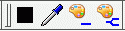
\includegraphics[width=3cm]{images/color-buttons.png}
        \end{center}    
\end{itemize}
The first button (black in the graphic above) shows the current colour.
Clicking on it let's you choose another colour. You can also "pick"
another colour by selecting a branch with the desired colour and using
the "pick colour" button. Both of the icons showing a palette actually
apply the current colour to the selected branch. While the first one
just colours the heading of the selection, the last one also colours all
the children of the selected branch.

%tipp
A very useful function is the {\em pick color modifier} of the mouse:
Select the branch which should get the new colour, then press
\key{Shift} and simultanously click with left-mouse on another branch to
copy its colour to the currently selected subtree. If you only want to
color the branch, not the whole subtree, press \key{Shift}+\key{Ctrl}
simultanously. 

\subsubsection*{Use flags}
\vym provides various flags. They are usually displayed in the toolbar
on top of the mapeditor window. (Note: Like all toolbars you can also
move them to the left or the right side of the window or even detach
them. Just grab the very left "dotted" part of the toolbar with your
left-mouse button.) 
\maximage{images/default-flags.png} 
If you have a branch selected, you can set any number of flags by
clicking them in the toolbar. The toolbar buttons change their state and
always reflect the flags set in the selected branch. So, to remove a
flag from a branch, select the branch and then click the highlighted
flag on the toolbar.

\vym uses three kinds of flags: 
\begin{itemize}
    \item {\em System Flags}
        are set by \vym to indicate e.g. that there is additional
        information in a note (more on this in \ref{noteeditor}) or 
        that there is a task associated (see the \ref{taskeditor})
    \item {\em Standard Flags}
    \item {\em User Flags} 
\end{itemize}
Standard flags can be toggled by clicking in the toolbar
    \maximage{images/default-flags.png}
User flags are similar, but can be added to their own toolbar when clicking the edit icon

\subsubsection*{Images}
The easiest way to add an image to a branch is by dragging it e.g. from a
webbrowser to the mapeditor while a branch is selected there.

You can also add an image to a branch by opening the context menu of the
branch. Right click the selected branch, choose "Add Image". A dialog
window enables you choose the image to load. 
\footnote{Supported image types are: PNG, BMP, XBM, XPM and PNM. It may
    also support JPEG, MNG and GIF, if specially configured during
    compilation (as done when \vym is part of SUSE LINUX).}
While an image is selected in the dialog, a preview of the image is
displayed. It is also possible to select multiple images.  

You can position the image anywhere you want, just drag it with left
mouse. To relink it to another branch, press \key{Shift} while moving
it. To delete it, press \key{Del}. 

If you right-click onto an image, a context menu will open which let's
you first choose one of several image formats. Then a file dialog opens
to save the image. 

\hint{ This is used to "export" the image as separate file. As part of
the map it always will be
saved anyway in the map itself! You can also cut and
copy images.}
Note that it is not possible to add objects to an image, which would
make working with the map much more complex if e.g. images could be
linked to images.

The option "{\bf Use for export}" controls the output of exports
e.g. to HTML: If set to no, the image won't appear in the {\em text}
part of the output. This is useful for large images or if images are
used as a kind of frame e.g. the famous cloud symbol around a part of
the map. Those shouldn't appear in the middle of the text.

Resizing images has been added to /vym in version 1.13.20. Later
versions will include more functionality like 
changing its z-value (put it into background) etc.

\subsubsection*{Frames}
Various types of frame can be added to a branch in the {\em property window} (see
\ref{propwindow}), e.g. ellipses, rectangle and cloud. The frames can
optionally also include the children of the the framed branch, thus
allowing even to "put boxes of contents into other boxes".
Alternatively, you can use use images as frames: 
\maximage{images/frames.png}

\subsection{Design of map background and connecting links }
The design of the background of a map and also of the links connecting
various parts of the map can be changed by
\begin{itemize}
    \item Selecting Format from the menu
    \item Right clicking on the canvas, which will open a context menu
\end{itemize}

\subsubsection*{Background }
The colour is set (and also displayed) as "Set background colour".
Alternativily you can set a background image, though this is not
recommended in general. Working on the map becomes slow and the image
currently cannot be positioned freely.

\subsubsection*{Link colour}
Links connecting branches can be coloured in one of two ways:
\begin{itemize}
    \item use the same colour for the heading and for the branch link
    line.
    \item use {\em one} colour for all links and choose different
    colours for the branch headings text. The default colour for branch
    link lines is blue.
\end{itemize}
The latter can be set with "Set link colour". Check or uncheck the "Use
colour of heading for link" option to toggle between the two designs for
your map.

\subsubsection*{Link style}
\vym offers four different styles for the appearences of links:
\begin{itemize}
    \item Line
    \item Parabel
    \item Thick Line
    \item Thick Parabel
\end{itemize}
The "thick" styles only apply to links starting at the mapcenter, link
lines for the rest of the map are always painted "thin".

\subsection{Links to other documents and webpages}
\vym supports two kind of external links:
\begin{itemize}
    \item Documents, viewed with an external webbrowser.
    Examples are {\tt .pdf} and {\tt .html} files. References 
    are called {\em URLs} and marked with the globe
    flag:
    \begin{center}
	
\includegraphics[width=0.5cm]{images/flag-url.png}
    \end{center}

    \item \vym maps, viewed in \vym itself. References are called
    a {\em vymlinks} and marked with the \vym flag:
    \begin{center}
	
\includegraphics[width=0.5cm]{images/flag-vymlink.png}
    \end{center}
\end{itemize}

\subsubsection{How to create an URL} 
Use one of the following:
\begin{itemize}
\item{Drag and drop URL from a webbrowser}
\item{Use the "URLs and vymlinks toolbar:}
    \begin{center}
	
\includegraphics[width=0.5cm]{images/flag-urlnew.png}
    \end{center}
\item{Keyboard shortcut:}
    Press \key{U} or right-click  onto a
    branch to open the contextmenu then choose "References\ra Edit URL". If
    you want to use a file dialog to conveniently choose a local file you
    can use~\key{U}. Also drag and drop from a browser can be used to create
    a new branch with an URL.
\item{Context menu:} 
    Right click onto branch,
    in the context menu there is also an option to open all URLs found
    in the selected subtree of the map. That's useful to simultanously open
    a collection of URLs in the webbrowser, especially if the browser can
    open them in tabs.

\end{itemize}

After an URL was entered, a little globe will appear in the branch. By
clicking on the globe in the toolbar or the context menu an external
browser\footnote{
    The browser can be changed in the Settings Menu (see \ref{settings}).}
will be launched. You can also press \key{Ctrl} while clicking the
globe, to open the URL in a new tab.

For more information on working with bookmarks and webbrowsers see
section \ref{bookmarks}.

If your \vym installation supports accessing external tools like JIRA or
Confluence, \vym might update the branch after retrieving information
from the tool, e.g. replacing the complete URL of a Confluence by its
concrete page name. 
\subsubsection{How to create a vymlink}
Creation is possible both from the "URLs and vymlinks" toolbar or from
the context menu of a branch:
    \begin{center}
	
\includegraphics[width=0.5cm]{images/flag-vymlinknew.png}
    \end{center}

A file dialog opens where you can choose the map. 
Clicking this flag beside the branch heading, in the toolbar or in the
context menu of a branch will open the map in another tab (see
\ref{tabs} for working with multiple maps). To delete an existing link,
just right click the branch and select "Delete \vym link" or
alternatively press both \key{Shift}\key{Ctrl} while clicking the
vymlink.

\hint{Open a linked map in background by pressing \key{Ctrl} while
clicking on the icon in the map}

In the context menu there is also an option to open all vymlinks found
in the selected subtree of the map. That's useful to simultanously open
a collection of related maps\footnote{
    Technical note: Internally \vym uses absolute paths, to avoid
    opening several tabs containing the same map. When a map is saved,
    this path is converted to a relative one 
    (e.g. {\tt /home/user/vym.map} might become {\tt ./vym.map}. This
    makes it fairly easy to use multiple maps on different computers or
    export them to HTML in future.}.


\subsection{Multiple maps} \label{tabs}
You can work on multiple maps at the same time. Each new map is opened
in another {\em tab}. The available tabs are shown just above the
mapeditor. You can use the normal cut/copy/paste functions to
copy data from one map to another.

\subsection{Brainstorming} \label{brainstorming}
When brainstorming you collect quickly a number of thoughts or ideas,
without sorting, discussing or otherwise spending any amount of time on
a particular idea.

\vym helps you to quickly create mapcenter, either by pressing \key{C}
or clicking the 
    \begin{center}
	
\includegraphics[width=0.5cm]{images/newmapcenter.png}
    \end{center}
If you want to place the new  mapcenter at a specific position, you
could also open the context menu by right-clicking on the background and
selecting "Add mapcenter".

Once you are done adding new items, you can start to sort them and
arrange them by moving and relinking them to create a new map.

\hint{If you have enabled "Automatic Layout"\ in the Settings menu,
the new parts will move around to avoid overlapping}

%TODO
%\subsubsection{Menus}
%\subsubsection{Keyboard shortcuts}

% Settings
% Images
% Copy & Paste
% Working with tabs (multiple maps)
% Exporting
% Scrolling

\section{Noteeditor} \label {noteeditor}
If you want to attach more text to a branch e.g. a complete email, a
cooking recipe, or the whole source code of a software project, you can
use the noteeditor. (The {\em Headingeditor} has the same features.)
    \maximage{images/noteeditor.png}
This editor displays text associated with a branch selected in the
mapeditor. The noteeditor shows different background colours
depending on whether text is associated with a selected branch.

\subsection{States}
Before you can type or paste text into it, you have
to select a branch in the mapeditor.
In the mapeditor a little "notepad" flag will appear
next to the heading of the branch, once you have entered some text in
the noteeditor. This is illustrated in the lower
branch on the right hand side: 
\maximage{images/branches-flags.png}

\subsection{Import and export notes}
The note is always saved automatically within the \vym map itself.
Nevertheless sometimes it is nice to import a note from an external file
or write it. In the Note Editor use "File\ra~Import" and
"File\ra~Export" to do so. 

\subsection{Edit and print note}
Editing works like in any simple texteditor, including undo and redo
functions. You can delete the complete note by clicking the trashcan.
Only the note itself is printed by clicking the printer icon.

\subsection{RichText: Colours, paragraphs and formatted text}
Notes and also the headings of branches can either use a default font or
all text attributes availabe in RichText, like bold, italic, colors,
etc. To enable the latter, click the RichText button:
\begin{center}
    
\includegraphics[width=0.5cm]{../icons/formatrichtext.png}
\end{center}

\subsection{Fonts and how to switch them quickly}
If you just want to do quick notes and don't need fully formatted
RichText as mentioned above, you still can select either a fixed font
width font or a variable width font by clicking
\begin{center}
    
\includegraphics[width=0.5cm]{../icons/formatfixedfont.png}
\end{center}


The fixed font is usually used for emails, source code etc.\ while the
variable font is used for simple notes, where one doesn't need fixed
character widths.  

In the Settings menu both fonts can be set. The default font can also be
toggled between the fixed and variable font by selecting or deselecting
the "fixed font is default" menu item.

\hint{Additionally to the default fonts any font installed on your system can
be used. Please note, that the chosen font also will be used for HTML
exports, so if your VYM mind map should  be exported to a web page
you should only use fonts which are available generally.}

\subsection{Find text}
The noteeditor itself has no Find function, use Find in the mapeditor,
which will also display occurences of text in notes (see
\ref{findwindow}).

\subsection{Paste text into note editor}
Often you will paste text into the editor from another application e.g.
an email.

\section{Task editor} \label{taskeditor}
Tasks are used to easily create and maintain a "Todo-list". 
The taskeditor is visible on the left side in the image below. 
\begin{center}
    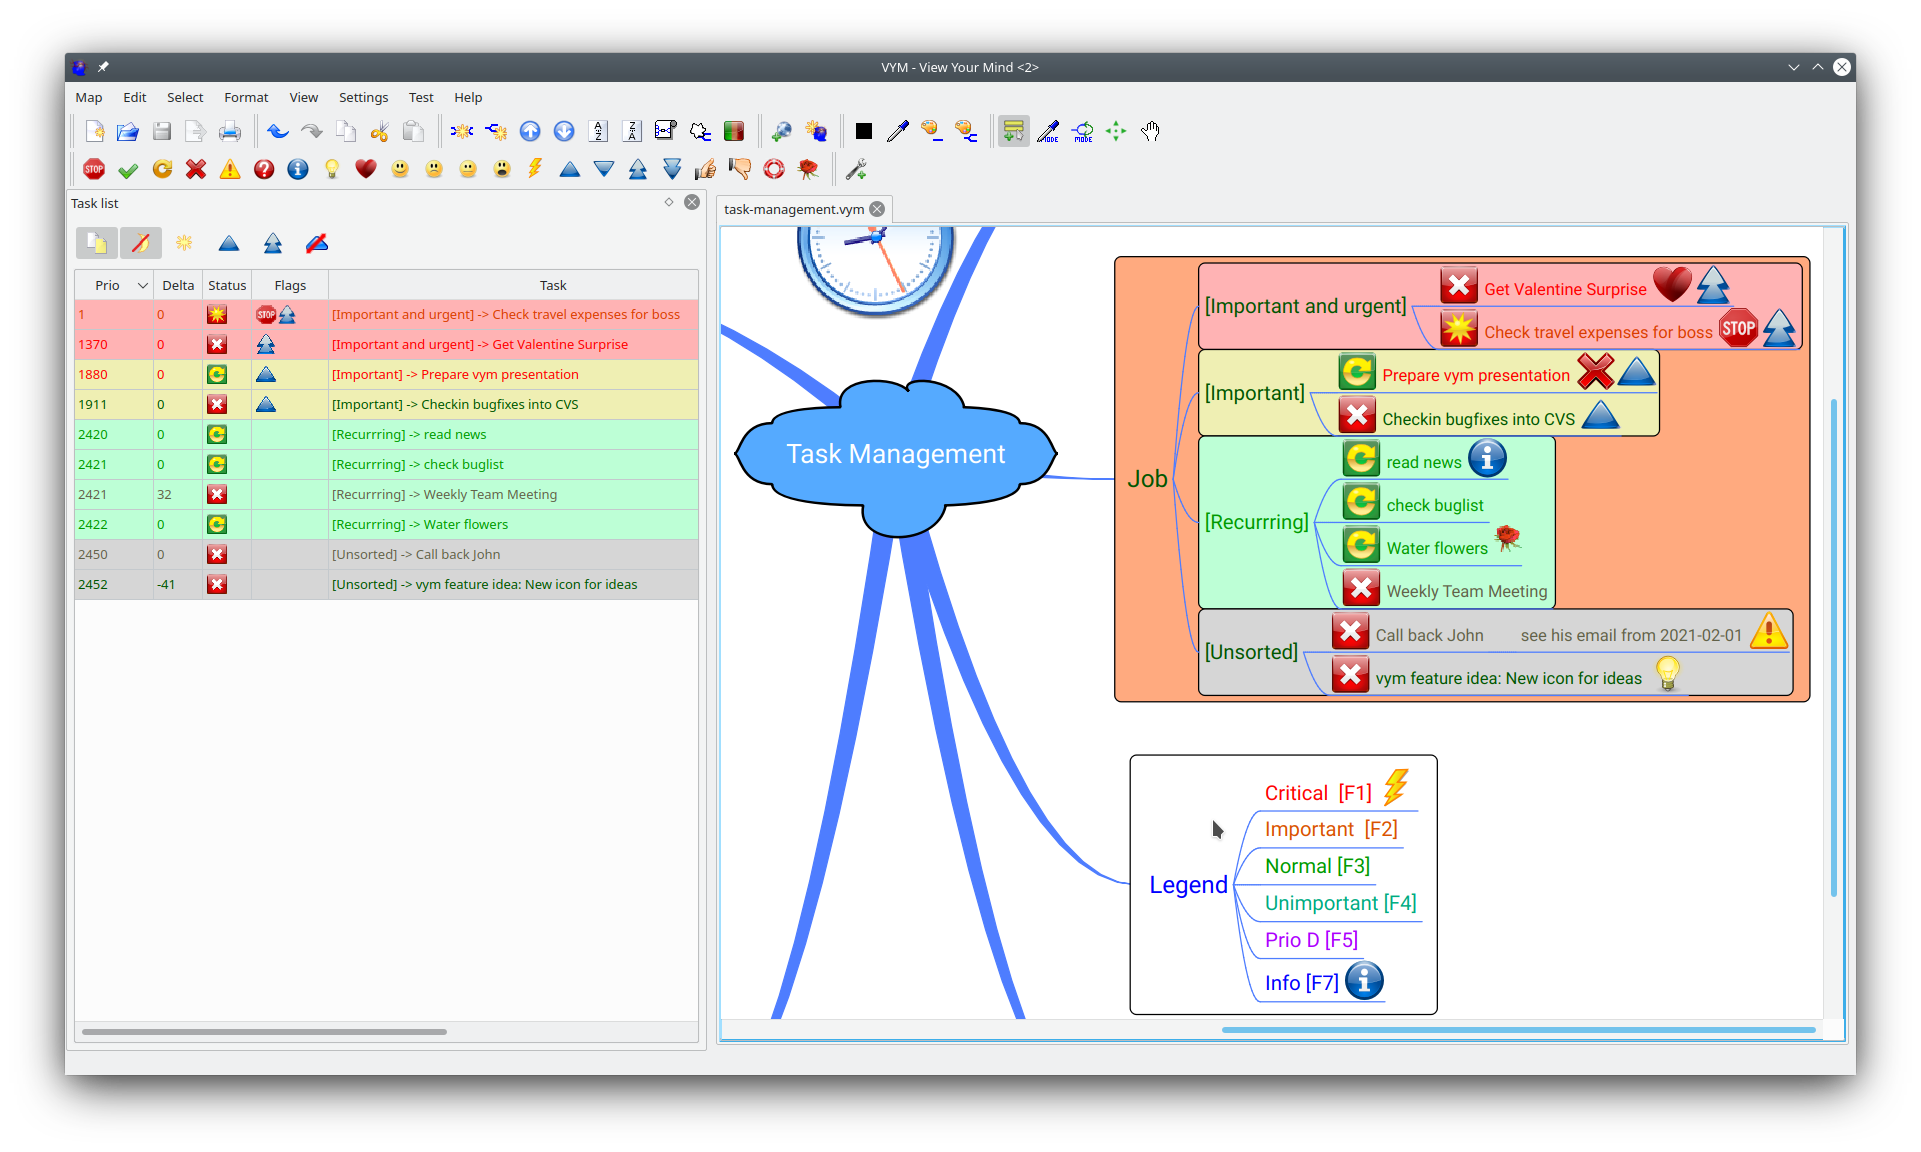
\includegraphics[width=13cm]{images/taskeditor.png}
\end{center}

The default columns in the taskeditor list are:
\begin{itemize}
    \item Delta: This value can be manually added to the priority to change the automated priorization
    \item Status: Shows the state and if the task is currently sleeping
%    \item Age total: Days, since the task has been created
%    \item Age modified: Days, since the task has been changed
%    \item Sleep: Days, which will pass until task will wake up 
%    \item Position of tasks branch in its subtree (higher priority if further up)
    \item Flags: Lists flags, which affect the priority (see above)
    \item The name of task (identical to heading of branch in the map)    
\end{itemize}
Priorities can be adjusted manually in the taskeditor, either by entering a
delta value or by dragging the task to a new position (more on priorities below).


\subsection{Creating tasks}
To create a task press \key{Shift + W}. The branch will get an
additional flag and its name will be visible in the taskeditor.

A task can have different states:
\begin{itemize}
    \item New task or just awakened task 
\includegraphics[width=0.5cm]{images/flags/system/task-new.png}
    \item Not started 
\includegraphics[width=0.5cm]{images/flags/system/task-not-started.png}
    \item Work in progress 
\includegraphics[width=0.5cm]{images/flags/system/task-wip.png}
    \item Finished 
\includegraphics[width=0.5cm]{images/flags/system/task-finished.png}
\end{itemize}
You can cycle these states by pressing \key{W}. 

\subsection{Reminders - let a task sleep for a while}
A task may be set to "sleep", which can be used to get a reminder
after a certain amount of time. The flag will change to one of these:
\begin{itemize}
    \item Not started - sleeping
    
\includegraphics[width=0.5cm]{images/flags/system/task-new-sleeping.png}
    \item Work in progress - sleeping
    
\includegraphics[width=0.5cm]{images/flags/system/task-wip-sleeping.png}
\end{itemize}
You can set the sleep time of a task should right clicking on the task flag in the
mapeditor or the task in the taskeditor. "Reset sleep" will wake up
a currently sleeping task. 

Alternatively you can press \key{Shift-Q} and manually enter the sleep time, here are some examples:

\begin{center}
    \begin{tabular}{|c|p{11cm}|} \hline
        {\bf Input }   & {\bf Sleep} \\ \hline
        1       & 1 day, postpone until tomorrow morning\\
        365     & 365 days \\
        1w      & 1 week \\
        3h      & 3 hours \\
        10s     & 10 seconds \\
        18:00   & Postpone until 6pm \\
        24.12.2024  & Postpone until Dec 24 in 2024 \\
        2024-12-24  & Postpone until Dec 24 in 2024 \\ 
        2038-12-24T21:34 &  Postpone until December 24 in 2038, 9:34 pm (ISO format)  \\ \hline
    \end{tabular}
\end{center}

%These tasks will get a  new flag and status
%in the taskeditor:
%\begin{itemize}
%    \item Not started - morning  %
\includegraphics[width=0.5cm]{../flags/flag-task-new-morning.png}
%    \item Work in progress - morning % 
\includegraphics[width=0.5cm]{../flags/flag-task-wip-morning.png}
%    \item New tasks - only show new freshly "woken up" tasks
%    \item Various filters for priorty flags
%    
\includegraphics[width=0.5cm]{../flags/flag-arrow-up.png}
%    
\includegraphics[width=0.5cm]{../flags/flag-2arrow-up.png}
%    
\includegraphics[width=0.5cm]{../flags/flag-no-arrow-up.png}
%    \ldots
%\end{itemize}

\subsection{Priority of tasks}
The tasks visible in the taskeditor are ordered by their {\em
priorities}, listed on the left side of the editor. The lower the
priority number, the more important is a task: The most important task always has priority~1.

There are several principles that influence the priority of a task:
\begin{itemize}
    \item
        Old tasks tend to bubble up, meaning theyget a higher priority over
        time. Rationale: If you have a task named "water the flowers"\ and
        you have postponed it now for 187 days, better delete the task. (And
        create a new task to dump the remains of the flowers.)

    \item
        Colors in the map: If you use the Function keys to assign the
        colors red, amber, green, etc. the tasks will get a different
        priority accordingly

    \item
        The stopsign flag
        
\includegraphics[width=0.5cm]{images/flags/stopsign.png} 
        will increase the priority. Use it for your shipstoppers\ldots

    \item
        The arrow up flags also move tasks up in the list 
        %FIXME add flag

    \item
        Sleeping tasks and finished tasks will tend to fall to the bottom of
        your task list.

    \item
        The freshly woken up "morning tasks"\ will tend to pop up right
        at the top, so that they cannot be missed. Remove the "morning"\ state by pressing \key{W} once.
\end{itemize}

\subsection{Filter tasks - keeping the overview}
The taskeditor has filters:  %FIXME add flag icons
\begin{center}
    \begin{tabular}{|c|p{11cm}|} \hline
        {\bf Icon} &   {\bf Filter }   \\ \hline
        
\includegraphics[width=0.4cm]{../icons/taskfilter-currentmap.png} &
             Current map only, hide tasks from other maps \\
        
\includegraphics[width=0.4cm]{../icons/taskfilter-activetask.png} &
            Active tasks only, hide finished nor sleeping \\
        
\includegraphics[width=0.5cm]{../icons/taskfilter-newtask.png} &
             New tasks only \\
        
\includegraphics[width=0.4cm]{images/flags/arrow-up.png}
        
\includegraphics[width=0.4cm]{images/flags/arrow2-up.png} &
            Tasks with "arrow up" flags only        \\
        
\includegraphics[width=0.4cm]{../flags/system/no-arrow-up.png} &
            Only tasks without "arrow up" flags \\ \hline
    \end{tabular}
\end{center}


\section{Slideeditor - presentations}\label{slideeditor}
\vym can be used to do animated presentations using the slideeditor as
seen on the right side of the image below:
\begin{center}
    
\includegraphics[width=13cm]{images/slideeditor.png}
\end{center}
The slideeditor can be opened by pressing \key{S} or from the {\em View}
menu. The (currently) available action are:
\begin{itemize}
    \item
    
\includegraphics[width=0.5cm]{../icons/slideprevious.png}
    Select previous slide

    \item
    
\includegraphics[width=0.5cm]{../icons/slidenext.png}
    Select next slide

    \item
    
\includegraphics[width=0.5cm]{../icons/slide-camera.png}
    Create a new slide by snapshotting the current selection. The exact
    set of actions performed when selecting the new snapshot defined in
    a script called {\tt slideeditor-snapshot.vys}. The script is one of
    the \vym macros, see \ref{macros}.

    \item
    
\includegraphics[width=0.5cm]{../icons/scripteditor.png}
    Open the scripteditor to manually edit the current slide \\
    (More on scripting in appendix \ref{scripts}).
    
    \item
    
\includegraphics[width=0.5cm]{../icons/edittrash.png}
    Delete the current slide
    
    \item
    
\includegraphics[width=0.5cm]{../icons/up.png}
    Move current slide up in slidedeck
    
    \item
    
\includegraphics[width=0.5cm]{../icons/down.png}
    Move current slide down in slidedeck
\end{itemize}
In the {\em View-menu} or it's toolbar you can also toggle the
presentation mode to hide most of the toolbars and buttons


\section{Hello world - vym and other applications}
This section is about how \vym can interact with other applications.
Many applications can now read and write their data using XML, the
eXtensible Markup Language. \vym also uses XML to save its maps, see
\ref{fileformat} for a more detailed description. 

So if you make use of another application that understands XML, chances
are good that someone could write import/export filters for \vym.
Volunteers are always welcome ;-)

\subsection{Import} \label{import}

\subsubsection{Mozilla Firefox bookmarks}
Currently \vym supports an experimental import of Firefox bookmarks:
Firefox can backup bookmkarks in a file in JSON format. This file can be
imported into an existing \vym map.

Future \vym versions might be able to export this bookmark map again to JSON, so
that it could be restored in Firefox.

\subsubsection{Freemind and Freeplane}
Freemind is no longer actively developed, the project is continued in
the Freeplane project, see also
\href{https://www.freeplane.org/}{https://www.freeplane.org/}.

\vym supports reading the general structure of a Freeplane map and some
of its flags. Also notes are read.

\subsubsection{Mind Manager}
\vym has currently a very basic import filter to convert maps created by
{\em Mind Manager}\footnote{Mind Manager is a commercial i.e. non free,
software application by Mindjet for Windows and the Mac. Both names are
registered trademarks by Mindjet. For more information see their website
at \href{http://mindjet.com}{http://mindjet.com}} into \vym maps. Notes
and pictures are not converted at the moment. You can import files with
\begin{itemize}
    \item File \ra Import\ra Mind Manager
\end{itemize}


\subsubsection{Directory structure}
\vym can read a directory structure. This is mainly for
testing \vym e.g. to easily create huge maps used for benchmarks (yes,
there is still room to optimize \vym ;-)

\subsection{Export}  \label{export}
\label{hideexport}
Often you may not want to export the whole map, but just parts of it.
For example you may have additional info you want to talk about in a
presentation, while those parts should not be visible to the audience.
To achieve this you can "hide" parts of the map during exports by
setting the "hide in export" flag.
\begin{center}
    
\includegraphics[width=0.5cm]{images/flag-hideexport.png}
\end{center}
You can toggle this flag in the toolbar or by pressing \key{H}.  Note
that there is a global option in the settings menu ( \ref{settings}) to
toggle the use of this flag. By default the flag is enabled.

\subsubsection{Last used format}
Repeats the last export action without further dialogs like asking for
directories. The associated export type and filepaths are stored within
the map and thus map specific. Note: Not all export types support this
feature yet.

\subsubsection{Image}
\vym supports all image formats which are natively supported by the
QT~toolkit:
BMP, JPEG, PBM, PGM, PNG, PPN, XPM, and XBM.
For use in websites and for sending images by email PNG is a good
recommodation regarding quality and size of the image. \vym uses QTs
default options for compressing the images.

\subsubsection{PDF}
Exports to Portable Document Format.

\subsubsection{SVG}
Exports to Scalable Vector Graphics.

\subsubsection{Open Office}
Open Office beginning with version~2 uses the so called "Open Document
Format", which can be written by \vym. The options are currently
limited, but it possible to export presentations which can be opened in
Open Office Impress. By selecting
\begin{itemize}
    \item File  \ra Export\ra Open Office
\end{itemize}
you get a file dialogue where you can choose the output file and the
file type:
    \maximage{images/export-oo.png}
The file types represent various templates, which can be created with
some manual work from an existing Open Office document. The structure of
\vym map is then inserted into a template.  There are some limitations
at the moment:
\begin{itemize}
    \item \vym can't take care of page lengths, so you have to check and
    probably reedit in Open Office to avoid text running over the end of
    a page
    \item Images and flags are not used at the moment
    \item Notes are just written as plain text, without RichText 
    \item The full range of templates are not available in all
    distributions.   
\end{itemize}
Some of the templates make use of {\em sections} i.e sections insert the
headings of mainbranches as chapters for sections into the presentation.

\subsubsection{HTML (Webpages)}
This is the format to use if you wish to create a webpage. To see an example
visit the \vym homepage: 
\href{http://www.InSilmaril.de/vym}{www.InSilmaril.de/vym}
A dialog allows the user to set various options:
\begin{itemize}
    \item {\bf Include image:} If set, \vym will create an image map at
    the top of the HTML output. Clicking on a branch in the map will
    jump to the corresponding section in the output.

    \item {\bf Colored headings:}
    If set to yes, \vym will colour the headings in the text part  with the
    same colours used in the \vym map.
    \item {\bf Save settings:}
    If set to yes, \vym will save above settings in the map.
\end{itemize}

\subsubsection{A \& O -- Achievements and Objectives}
A specialized form of ASCII export (see next section), which is used for
workreports. Currently it is considered experimental.
%FIXME-3 Details

\subsubsection{ASCII}
Exporting a map as text is somewhat experimental at the moment. Later
this will probably be done using stylesheets. So the output may change
in future versions of \vym.

\subsubsection{CSV}
Exports map into a Comma Separated Value file, which can be used to
import into all kinds spreadsheet software.

\subsubsection{Taskjuggler}
Used to export to Taskjuggler project management software. Currently
considered experimental.

\subsubsection{\LaTeX}
\vym can generate an input file for \LaTeX. Currently this is considered
as experimental, there are no options (yet). 
By selecting
\begin{itemize}
    \item File  \ra Export\ra \LaTeX 
\end{itemize}
you will be asked in a file dialog for the name of the output file. This
file may then be included in a \LaTeX document using command: 
\begin{verbatim}
    \include{inputfile.tex}
\end{verbatim}
New in version 2.2.0: You can configure the names of the sections in the
vym config file, depending on your platform e.g. in 
\begin{verbatim}
    $HOME/.config/InSilmaril/vym.conf
\end{verbatim}
Just add e.g. these entries>
\begin{verbatim}
    /export/latex/sectionName-0=chapter
    /export/latex/sectionName-1=section
    /export/latex/sectionName-2=subsection
    /export/latex/sectionName-3=subsubsection
    /export/latex/sectionName-4=paragraph
\end{verbatim}

\subsubsection{Markdown}
Used to export to Markdown, see also
\href{https://daringfireball.net/projects/markdown/}{https://daringfireball.net/projects/markdown/}
Currently considered experimental.

\subsubsection{OrgMode}
Used to export to Emacs OrgMode, see also
\href{https://orgmode.org/}{https://orgmode.org/}
Currently considered experimental.


\subsubsection{XML} \label{xmlexport}
The map is written into a directory both as an image and as an XML file.
The directory is set in a file dialog. If the directory is not empty,
you will be warned and offered choices if you are at risk of overwriting
existing contents.

It is possible to export different maps into the same directory. Each
file generated will have the map's name as prefix, e.g. {\tt todo.vym}
becomes {\tt todo.xml}, {\tt todo.png}, {\tt todo-image-1.png} and so
on. This is useful if, for example, a website comprises several combined
maps that have to be stored in the same directory.

\subsubsection{Export a part of a map}
Select a branch you want to export together with its children, then open
the context menu and choose {\em Save Selection}. This will create a
file with the suffix {\tt .vyp}, which is an abbreviation for "vym
part".

\subsection{Connect vym to the cloud}  \label{cloud}
Starting with \vym 2.8.16 some exchange with cloud applications is
possible. So far this is limited to cloud applications from the company
Atlassian\footnote{Atlassian, Confluence and JIRA are registered
trademarks}. You find the related features and settings in the "Connect"
settings in the menubar on top of the main window.
\subsubsection{Confluence}
\vym so far can
\begin{itemize}
    \item Get Confluence user name and insert it into map. (This will
        create a link to the user profile during export to Confluence)
    \item Export a map to a Confluence page
    \item Get the name of a Confluence page and the space name and use
        it as heading when pasting an URL. (Happens automatically, if
        Confluence is configured)
\end{itemize}

\subsubsection{JIRA}
\begin{itemize}
    \item Get description of a JIRA ticket and use it as heading
    \item Get additional information, e.g. color branch if ticket is
        already closed
\end{itemize}

\subsection{Connect vym using DBUS}
If you don't know what DBUS is, you probably want to skip this section,
this is about remote controling \vym using the DBUS protocol on Linux.

Currently this is used to
\begin{itemize}
    \item Run the development tests, see also 

        \href{https://github.com/insilmaril/vym/blob/develop/test/vym-test.rb}
        {https://github.com/insilmaril/vym/blob/develop/test/vym-test.rb}
    \item Add content from other applications, e.g. paste an email from
        the mutt client, see also 

        \href{https://github.com/insilmaril/vym/blob/develop/scripts/vym-addmail.rb}
        {https://github.com/insilmaril/vym/blob/develop/scripts/vym-addmail.rb}
\end{itemize}
For more details see also \ref{dbus}.

\section{Advanced usage}

\subsection{Quickly sorting branches or postponing actions} \label{targets}
Sometimes it's very handy to have a small number of shortcuts to quickly
select a certain branch or move something somewhere and proceed with
next item. This can be used for quick sorting to a number of
destination. For example if used in timeplanning, you could quickly move something
to "next tuesday". The destinations are called {\em targets} and are
marked with 
\begin{center}
    
\includegraphics[width=0.5cm]{images/flag-target.png}
    \label{propwindow}
\end{center}
The target flag is toggled with \key{T}. If you want to "Goto" a target,
press \key{G}. Similar if you want to "Move" a branch, press \key{M}.
A context menu will open and lets you select the target.



\subsection{Properties of an object} 
For any branch you can open a satellite window (see \ref{satellite}):
the {\em property window}:
\begin{center}
    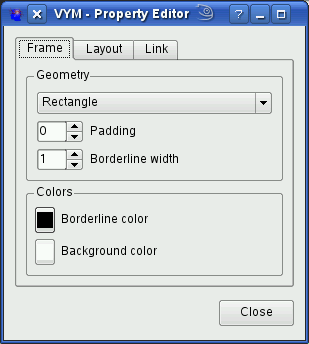
\includegraphics[width=8cm]{images/propwindow.png}
    \label{propwindow}
\end{center}
%FIXME create updated screenshot

\subsubsection*{Frame}
sets the appearance of the frame of a branch. Currently there are
\begin{itemize}
    \item No frame
    \item Rectangle
    \item Ellipse
    \item Cloud
\end{itemize}
The "Include Children" checkmark is used to, well, include the children
of the branch. "Padding" sets the distance between both neighbouring
branches and frame and also the frame and branch itself. The "width"
sets the thickness of the frame.

Two colors can be assigned to background of the frame and frame itself.

\subsubsection*{Layout}
The images belonging to a branch can use different layouts, e.g.
floating freely alongside or being included {\em within} the branch. For
details and illustration see \ref{incimg}).

\subsubsection*{Link}
The advantage of hiding a link, which is the connection between a branch
(or image) and its parent, is to make the branch itself appear a
mapcenter of its own. Details are in   \ref{hidelink}).

\subsection{Changing the history: Undo and Redo}
\vym keeps track of all changes done in a map. The default number of
changes which can be undone is~75. The complete history can be seen in
the {\em historywindow}:
    \maximage{images/historywindow.png}
    \label{historywindow}
A single step back be undone or redone with \key{CTRL-Z} or \key{CTRL-Y},
or by using the buttons in the toolbar or the {\em historywindow}.
Inside the {\em historywindow}, you can click on a line to unwind all
actions done until that point in time -- or redo all changes by clicking
on the last line.

\hint{
    You can "paste from the past": Go back in time by e.g. with
    \key{CTRL-Z}, then copy to clipboard by pressing \key{CTRL-C}.

    Now do all actions again, e.g. by \key{CTRL-Y} or clicking on the
    last action in {\em historywindow}. Now paste from the past with
    \key{CTRL-V}.
}

\subsection{Macros} \label{macros}
Each function key
\key{F1} to \key{F12} holds a macro, which is executed on the current
selection if the key is pressed. The default macros change the colour of
a subtree or set the frame of a branch:
\begin{center}
    \includegraphics[width=8cm]{images/macros.png}
\end{center}
Each macro is a \vym script, which is executed when the associated key
is pressed. The default location of the scripts can be changed in the
Settings menu. More information on using scripts in \vym is found in
appendix~\ref{scripts}.

\subsection{Bookmarks} \label{bookmarks}
\subsubsection*{Open new tabs instead of new windows}
If you use konqueror as your browser, \vym will remember the konqueror session which
was opened first by \vym. You can also press \key{Ctrl} and click to
open the link in a new tab.

\vym can also open a new tab in Mozilla or Firefox using the remote
command\footnote{
    \href{http://www.mozilla.org/unix/remote.html}{http://www.mozilla.org/unix/remote.html}}
of these browsers.

\subsubsection*{Drag and Drop}
If you want to keep bookmarks in a map, select a branch where you want
to add the bookmark, then simply drag the URL from your browser to the
map. Also you could use an existing heading as URL: Right click onto the
branch and select "Use heading for URL".


\subsubsection*{Directly access bookmark lists of a browser}
Please see the sections \ref{import} and \ref{export} about
Import and Export filters.

\subsection{Associating images with a branch} \label{incimg}
The default setting for an image is for it to float "freely". Images can
be positioned anywhere on the canvas, but may end up in the same place
as other parts of the map obscuring that part of the map.

The solution is to insert or include them "into" a branch. This can be
done via the property window (see \ref{propwindow}):
\begin{itemize}
    \item Include images horizontally
    \item Include images vertically
\end{itemize}
The image is still positioned relative to its parent branch, but the
heading and border of the branch frame adapt to the floating image, see
below: \maximage{images/includeImages.png}

\subsection{Modifier Modes} 
The modifier mode can be selected in the toolbar
\begin{center}
    \includegraphics[width=3cm]{images/modmodes.png}
\end{center}
or also using the adjacent keys \key{L}, \key{K} and \key{L}.
The selected mode influences mouse behaviour when the \key{Shift}-modifier is
used:
\begin{itemize}
    \item Multiple selection: Press Shift and click to select multiple objects
    \item Colorpicker: Pick from another branch and apply to currently
        selected branch
    \item XLink: Draw a connecting XLink between two branches. See also
        \ref{xlinks}
    \item Move object: Move an object, but when releasing it over another one, do not relink.
        (Useful for positioning branches in other branches for presentations.)
    \item Move view: Only move view without selecting an object
\end{itemize}

\subsection{Hide links of unselected objects} \label{hidelink}
Sometimes it would be useful to position a branch freely, just like a
mainbranch or an image. This is possible for all branches, you can use a
mainbranch and hide its connecting link to the mapcenter or hide the
link between a child branch and its parent. This can be used e.g. for
legends or a collection of vymLinks pointing to other maps:
\begin{center}
    \includegraphics[width=9cm]{images/hiddenlink.png}
\end{center}
To hide the link between a branch and its parent open the
\ref{propwindow} and check "Hide link if object is not selected" on
"Link" tab.


\subsection{XLinks} \label{xlinks}
So far all the data in the \vym map has been treelike. Using xLinks you
can link one branch to any other, just like attaching a rope between two
branches in a real tree. This is especially useful in complex maps,
where you want to have crossreferences which can not be displayed on the
same visible area of the {\em mapeditor} window. The following example
map still fits on one screen, but shows how data can be crosslinked. In
the graphics there is a link from a task (prepare a presentation) to
general information: 
\maximage{images/xlink-control.png}
Note that a xLink which points to a branch, that is not visible (because
it is scrolled), is just shown as a little horizontal arrow. In the
image above have a look at the "Screenshot"\ branch.

\subsubsection*{Create a xLink}
Choose the link mode from the modifier toolbar (by clicking the toolbar
icon or pressing \key{L}). Select the branch, where the xLink should
start. Press the modifier key \key{Shift} 
drag the mouse pointer to the branch where the link should end. (The
link is drawn to follow the mouse pointer). When you release the mouse
over a branch the xLink becomes permanent.

\subsubsection*{Modify or delete a xLink}
First select the link, either in the tree editor or by clicking the xLink
itself in the mapeditor.  A dialogue opens, where you can set colour,
width and also delete the xLink.

You can also move the control points of the link to change the curve and
change the appearance of the xlink by right clicking on one of
the control points:
\begin{center}
\includegraphics[width=6cm]{images/xlink-property.png}
\end{center}


\subsubsection*{Follow a xLink}
In a complex \vym map it sometimes comes in handy to be able to jump to
the other end of a xLink. You can do this by opening the context menu of
the branch and clicking on "Goto xLink" and selecting the xLink you
want to follow. Even easier is to click on the lower right end of a
branch -- a popup menu will show up with all xLinked branches. Click one
of them to jump to it.


\subsection{Adding and removing branches}
The context menu of a branch shows some more ways to add and delete data
e.g. you can delete a branch while keeping its children. The children
become linked to the parent of the previously removed branch.  Similar
branches can be inserted into existing maps. For keyboard shortcuts also
have a look at the context menu.

\subsection{Adding a whole map or a part of a map}
Select a branch where you want to add a previously saved map ({\tt
.vym})or a part of a map ({\tt .vyp}) , then open the context menu and
choose {\em Add \ra Add Map (Insert)}. For the import you can choose
between {\em Add Map (Insert)} and {\em Add Map (Replace)}: The imported
data will be added after the selected branch.

\section{\vym on Mac OS X}
%FIXME-3 Currently not yet supported on Mac OS X in 1.13.x

%\subsection{Overview}
%Sorry, currently (\vym 2.2.2) there is no Mac port available. Please
%contact the author\footnote{
%    Email Uwe Drechsel: \href{mailto:vym@insilmaril.de}{vym@insilmaril.de}} if
%you are interested in a Mac version.

%Basically there are two ways to run \vym on Macs:
%\subsubsection*{Qt Mac Edition:}
%    \vym here provides the well known Mac look and feel.  \vym is
%    available as Mac OS X application package in contained in a disk
%    image ({\tt vym.dmg}). It has been compiled and tested in
%    Mac~OS~10.4.  This package includes  runtime libraries of Qt by
%    Trolltech.
    
%\subsubsection*{X11 version} \vym can also be run using the Linux
%version, but then menus and handling will also be those of the Linux
%version e.g. The menu bar will look different. 

\subsection {Contextmenu and special keys}
Most Macs unfortunatly just have a single mouse button. In order to show
the context menu which usually would be opened with the right mouse
button, you can click while pressing the \key{kommand}-key.

Especially on Laptops some of the keys usually used on PC keyboards seem
to be missing. The Qt-Mac Edition of \vym has its own keyboard
shortcuts. To find the shortcuts just have a look at all the menu
entries, the shortcut is visible next to an entry. Toolbar buttons also
may have shortcuts, just position the mouse pointer over a button and
wait for the little help window to appear. 

\subsection {Viewing external links}
\vym on Mac uses the system call {\tt /usr/bin/open} to view links.
Mac~OS determines automatically if the link is a pdf or www page and
opens the right browser.

\newpage

\begin{appendix}

\section{\vym initialisation process and configuration}
\subsection {Settings menu} \label{settings}
    The {\em Settings} menu allows to configure \vym to your needs:

\subsubsection*{Set application to open PDF files} Choose a PDF
    viewer like {\tt acrobat} or {\tt konqueror} which is installed on
    your system.

\subsubsection*{Set application to open external links}
    Choose your favourite application, this usually depends on your
    platform, e.g.
    \begin{enumerate}
        \item Windows: {\tt explorer}
        \item Linux: {\tt xdg-open} or {\tt mimeopen}
        \item Mac: {\tt /usr/bin/open}
    \end{enumerate}
    Defaults should be set by \vym automatically.

\subsubsection*{Set path for macros}
    Set the default search path for macros, which will be executed when
    you press one of the function keys. Each key corresponds to a file
    ({\tt macro-1.vys..macro12.vys}) in the search path.

\subsubsection*{Set number of undo levels}
    Sets the number of undo/redo levels. The default setting is
    75~levels.

\subsubsection*{Autosave and autosave time}
    Automatic saving of modified maps can be toggled on or off. The
    autosave time is entered in seconds.

\subsubsection*{Write backup on save}
    When saving a map called {\tt example.vym}, \vym will rename the
    existing file to {\tt example.vym\~{}} before writing the {\tt
    example.vym} itself.

\subsubsection*{Edit branch after adding it}
    If set, the heading of a new branch will be edited immediately after
    adding the branch.

\subsubsection*{Select branch after adding it}
    If set, a new branch will be selected immediately after adding it.
    When you "brainstorm" on a given keyword, you don't want to go
    deeper and deeper into details, but keep the focus on the keyword.
    So the default setting here is to {\em not} select the freshly added
    branch.
    
\subsubsection*{Select existing heading}
    If set and you begin to edit the heading of a branch, the heading
    text in the dialog will be selected. Usefully to copy\&paste to
    other applications.

\subsubsection*{Delete key}
    If set, the \key{Delete} is enabled to, well, delete objects. This
    can be switched off to avoid confusing with the nearby
    \key{Insert}-key on PC keyboards.

\subsubsection*{Exclusive flags}
    If set, some of the standard flags can only be used exclusively,
    e.g.~the smileys.

\subsubsection*{Use hide flags}
    If set, every branch which also has the hide flag set (see
    \ref{hideexport}) will be hidden in exports.

\subsubsection*{Note editor is dockable}
    If set (default), the note editor can be docked into the main
    widget. Changing this setting needs a restart of \vym. Details see
    \ref{dockable}.

\subsubsection*{Animation}
    If set (default), some animation will be used, e.g.\ for "snapping
    back" of released branches.

\subsubsection*{Autolayout} %FIXME-3
    If set (not on default), \vym will try to autolayout mainbranches.
    Currently considered experimental and only working under certain
    circumstances. 

\subsection{Configuration file}
On startup \vym will look for a configuration for user specific settings
like window positions, toolbars etc. If this file does not already
exist, it will be created. The file is located in the users home
directory. The exact position depends on the platform:
\begin{center}
\begin{tabular}{ll}
    {\bf Platform}  & {\bf Configuration file} \\ \hline
    Linux              & {\tt $\sim$/.config/InSilmaril/vym.conf  } \\
    Mac OS X           & {\tt /Users/NAME/Library/Preferences/com.insilmaril.vym.plist  } \\
    Windows (registry) & {\tt HKEY\_Current\_User/Software/InSilmaril/vym  } \\
\end{tabular}
\end{center}
The file can be edited manually, or on Mac~OS~X with Property List
Editor (installed with xtools). On windows you can use {\tt regedit.exe}.

\subsection{Path to resources}
\vym will try to find its resources (images, stylesheets, filters,
etc.) in the following places:
\begin{enumerate}
    \item Path given by the environment variable {\tt VYMHOME}.
    \item If called with the local option (see \ref{options} below),
          \vym will look for its data in the current directory.
    \item {\tt /usr/share/vym}
    \item {\tt /usr/local/share/vym}
\end{enumerate}

\subsection{Command line options} \label{options} 
\lstinputlisting{help.tex}
You can also give several filenames at the commandline to let \vym open
several maps at once.
 

\section{Scripts} \label{scripts}   
\subsection{Overview}
Beginning with version 2.7.0 \vym is fully scriptable, though the
scripting support is still considered a {\em technical preview}. Some
parts still might change and improve in later versions.
Scripts are internally used for
\begin{itemize}
    \item Undo and Redo
    \item Macros on function keys
    \item Slideshow
\end{itemize}
In addition to the internal scriptengine, which is using QScript, 
you can also  use external ruby scripts, which communicate with \vym via
DBUS. Please note that the latter is currently only possible on Linux.
See also the examples in \ref{examplescripts}.

The scripts within \vym are edited using the {\em script editor}:
\begin{center} \label{scripteditor}
    \includegraphics[width=13cm]{images/scripteditor.png}
\end{center}
Open the scripteditor by pressing \key{Alt + S} or from the {\em
View}-menu. The output of of scripts cans be seen in the script output
window with \key{Alt + Shift + S}

\subsection{Example scripts}  \label{examplescripts}
A set of example scripts is installed together with \vym, see the
installation directory and the subfolder {\tt demos/scripts/} and the
macros in the macro tab of the script editor.
\subsubsection{Macro to create a rounded rectangle frame}
\begin{code}
// Macro Shift + F1: Frame background light red
function macro_shift_f1()
{
    map = vym.currentMap();
    status = "Background off";
    if (map.getFrameType() == "NoFrame") {
        status = "Background light red";
    }
    toggle_frame ( map );
    map.setFrameBrushColor("#ffb3b4");
    statusMessage(status);
}
\end{code}

\subsubsection{Batch script to export all maps as images}
This script can be used to export all maps in a directory
automatically. If the script is named {\tt export-image.vys}, call \vym
with
\begin{code}
\$ vym --quit --run export-image.vys *.vym
\end{code}

\subsubsection{Full scripting using ruby and DBUS} \label{dbus}
Nearly every action in \vym can be controlled via DBUS (on Linux
machines). You can have several \vym instances running at the same time,
e.g. for production and development. Before controlling one, you need to
give it a name, here "test"\ is used:
\begin{verbatim}
vym -n test
\end{verbatim}
You can now access \vym via DBUS, if you have Qt installed, try {\tt
qdbusviewer}. In the {\tt scripts} directory, which is part of \vym,
you'll find the script {\tt vym-ruby.rb}. This rubyscript provides two
classes to manage and control \vym instances. A short script to set the
heading of a branch might be:
\begin{verbatim}
#!/usr/bin/env ruby

require "#{ENV['PWD']}/scripts/vym-ruby"

vym_mgr=VymManager.new
vym=Vym.new(vym_mgr.find('test') )

vym.select "mc:0"
vym.setHeading "This is a new heading!"
\end{verbatim}

An full example how this is
used is in the automated \vym testing:
\begin{verbatim}
test/vym-test.rb
\end{verbatim}

\subsection{Available commands}
Start vym with the "command"\ option to get a listing of available
commands:
\begin{verbatim}
  vym --commands --quit
\end{verbatim}
The currently available commands are:
\begin{itemize}
    \item addBranch\\
\begin{tabular}{rl}
  Selection: & Branch\\
   Parameter: &  0:\\
        Comment: & Index of new branch\\
           Type: & Int\\
       Optional: &  yes\\
\end{tabular}

\item addBranchBefore\\
\begin{tabular}{rl}
  Selection: & Branch\\
\end{tabular}

\item addMapCenter\\
\begin{tabular}{rl}
  Selection: & Any\\
   Parameter: &  0:\\
        Comment: & Position x\\
           Type: & Double\\
       Optional: &  No\\
   Parameter: &  1:\\
        Comment: & Position y\\
           Type: & Double\\
       Optional: &  No\\
\end{tabular}

\item addMapInsert\\
\begin{tabular}{rl}
  Selection: & Any\\
   Parameter: &  0:\\
        Comment: & Filename of map to load\\
           Type: & String\\
       Optional: &  No\\
   Parameter: &  1:\\
        Comment: & Index where map is inserted\\
           Type: & Int\\
       Optional: &  yes\\
   Parameter: &  2:\\
        Comment: & Content filter\\
           Type: & Int\\
       Optional: &  yes\\
\end{tabular}

\item addMapReplace\\
\begin{tabular}{rl}
  Selection: & Branch\\
   Parameter: &  0:\\
        Comment: & Filename of map to load\\
           Type: & String\\
       Optional: &  No\\
\end{tabular}

\item addSlide\\
\begin{tabular}{rl}
  Selection: & Branch\\
\end{tabular}

\item addXLink\\
\begin{tabular}{rl}
  Selection: & BranchLike\\
   Parameter: &  0:\\
        Comment: & Begin of XLink\\
           Type: & String\\
       Optional: &  No\\
   Parameter: &  1:\\
        Comment: & End of XLink\\
           Type: & String\\
       Optional: &  No\\
   Parameter: &  2:\\
        Comment: & Width of XLink\\
           Type: & Int\\
       Optional: &  yes\\
   Parameter: &  3:\\
        Comment: & Color of XLink\\
           Type: & Color\\
       Optional: &  yes\\
   Parameter: &  4:\\
        Comment: & Penstyle of XLink\\
           Type: & String\\
       Optional: &  yes\\
\end{tabular}

\item branchCount\\
\begin{tabular}{rl}
  Selection: & Any\\
\end{tabular}

\item centerCount\\
\begin{tabular}{rl}
  Selection: & BranchLike\\
\end{tabular}

\item centerOnID\\
\begin{tabular}{rl}
  Selection: & Any\\
   Parameter: &  0:\\
        Comment: & UUID of object to center on\\
           Type: & String\\
       Optional: &  No\\
\end{tabular}

\item clearFlags\\
\begin{tabular}{rl}
  Selection: & BranchLike\\
\end{tabular}

\item colorBranch\\
\begin{tabular}{rl}
  Selection: & Branch\\
   Parameter: &  0:\\
        Comment: & New color\\
           Type: & Color\\
       Optional: &  yes\\
\end{tabular}

\item colorSubtree\\
\begin{tabular}{rl}
  Selection: & Branch\\
   Parameter: &  0:\\
        Comment: & New color\\
           Type: & Color\\
       Optional: &  yes\\
\end{tabular}

\item copy\\
\begin{tabular}{rl}
  Selection: & BranchOrImage\\
\end{tabular}

\item cut\\
\begin{tabular}{rl}
  Selection: & BranchOrImage\\
\end{tabular}

\item cycleTask\\
\begin{tabular}{rl}
  Selection: & BranchOrImage\\
   Parameter: &  0:\\
        Comment: & True, if cycling in reverse order\\
           Type: & Bool\\
       Optional: &  yes\\
\end{tabular}

\item exportMap\\
\begin{tabular}{rl}
  Selection: & Any\\
   Parameter: &  0:\\
        Comment: & Format (AO, ASCII, CONFLUENCE, CSV, HTML, Image, Impress, Last, LaTeX, Markdown, OrgMode, PDF, SVG, XML)\\
           Type: & String\\
       Optional: &  No\\
\end{tabular}

\item getDestPath\\
\begin{tabular}{rl}
  Selection: & Any\\
\end{tabular}

\item getFileDir\\
\begin{tabular}{rl}
  Selection: & Any\\
\end{tabular}

\item getFileName\\
\begin{tabular}{rl}
  Selection: & Any\\
\end{tabular}

\item getFrameType\\
\begin{tabular}{rl}
  Selection: & Branch\\
\end{tabular}

\item getHeadingPlainText\\
\begin{tabular}{rl}
  Selection: & TreeItem\\
\end{tabular}

\item getHeadingXML\\
\begin{tabular}{rl}
  Selection: & TreeItem\\
\end{tabular}

\item getMapAuthor\\
\begin{tabular}{rl}
  Selection: & Any\\
\end{tabular}

\item getMapComment\\
\begin{tabular}{rl}
  Selection: & Any\\
\end{tabular}

\item getMapTitle\\
\begin{tabular}{rl}
  Selection: & Any\\
\end{tabular}

\item getNotePlainText\\
\begin{tabular}{rl}
  Selection: & TreeItem\\
\end{tabular}

\item getNoteXML\\
\begin{tabular}{rl}
  Selection: & TreeItem\\
\end{tabular}

\item getSelectionString\\
\begin{tabular}{rl}
  Selection: & TreeItem\\
\end{tabular}

\item getTaskPriorityDelta\\
\begin{tabular}{rl}
  Selection: & Branch\\
\end{tabular}

\item getTaskSleep\\
\begin{tabular}{rl}
  Selection: & Branch\\
\end{tabular}

\item getTaskSleepDays\\
\begin{tabular}{rl}
  Selection: & Branch\\
\end{tabular}

\item getURL\\
\begin{tabular}{rl}
  Selection: & TreeItem\\
\end{tabular}

\item getVymLink\\
\begin{tabular}{rl}
  Selection: & Branch\\
\end{tabular}

\item getXLinkColor\\
\begin{tabular}{rl}
  Selection: & XLink\\
\end{tabular}

\item getXLinkWidth\\
\begin{tabular}{rl}
  Selection: & XLink\\
\end{tabular}

\item getXLinkPenStyle\\
\begin{tabular}{rl}
  Selection: & XLink\\
\end{tabular}

\item getXLinkStyleBegin\\
\begin{tabular}{rl}
  Selection: & XLink\\
\end{tabular}

\item getXLinkStyleEnd\\
\begin{tabular}{rl}
  Selection: & XLink\\
\end{tabular}

\item hasActiveFlag\\
\begin{tabular}{rl}
  Selection: & TreeItem\\
   Parameter: &  0:\\
        Comment: & Name of flag\\
           Type: & String\\
       Optional: &  No\\
\end{tabular}

\item hasNote\\
\begin{tabular}{rl}
  Selection: & Branch\\
\end{tabular}

\item hasRichTextNote\\
\begin{tabular}{rl}
  Selection: & Branch\\
\end{tabular}

\item hasTask\\
\begin{tabular}{rl}
  Selection: & Branch\\
\end{tabular}

\item importDir\\
\begin{tabular}{rl}
  Selection: & Branch\\
   Parameter: &  0:\\
        Comment: & Directory name to import\\
           Type: & String\\
       Optional: &  No\\
\end{tabular}

\item isScrolled\\
\begin{tabular}{rl}
  Selection: & Branch\\
\end{tabular}

\item loadImage\\
\begin{tabular}{rl}
  Selection: & Branch\\
   Parameter: &  0:\\
        Comment: & Filename of image\\
           Type: & String\\
       Optional: &  No\\
\end{tabular}

\item loadNote\\
\begin{tabular}{rl}
  Selection: & Branch\\
   Parameter: &  0:\\
        Comment: & Filename of note\\
           Type: & String\\
       Optional: &  No\\
\end{tabular}

\item moveDown\\
\begin{tabular}{rl}
  Selection: & Branch\\
\end{tabular}

\item moveUp\\
\begin{tabular}{rl}
  Selection: & Branch\\
\end{tabular}

\item moveSlideDown\\
\begin{tabular}{rl}
  Selection: & Any\\
\end{tabular}

\item moveSlideUp\\
\begin{tabular}{rl}
  Selection: & Any\\
\end{tabular}

\item move\\
\begin{tabular}{rl}
  Selection: & BranchOrImage\\
   Parameter: &  0:\\
        Comment: & Position x\\
           Type: & Double\\
       Optional: &  No\\
   Parameter: &  1:\\
        Comment: & Position y\\
           Type: & Double\\
       Optional: &  No\\
\end{tabular}

\item moveRel\\
\begin{tabular}{rl}
  Selection: & BranchOrImage\\
   Parameter: &  0:\\
        Comment: & Position x\\
           Type: & Double\\
       Optional: &  No\\
   Parameter: &  1:\\
        Comment: & Position y\\
           Type: & Double\\
       Optional: &  No\\
\end{tabular}

\item nop\\
\begin{tabular}{rl}
  Selection: & Any\\
\end{tabular}

\item note2URLs\\
\begin{tabular}{rl}
  Selection: & Branch\\
\end{tabular}

\item parseVymText\\
\begin{tabular}{rl}
  Selection: & Branch\\
   Parameter: &  0:\\
        Comment: & parse XML of VymText, e.g for Heading or VymNote\\
           Type: & String\\
       Optional: &  No\\
\end{tabular}

\item paste\\
\begin{tabular}{rl}
  Selection: & Branch\\
\end{tabular}

\item redo\\
\begin{tabular}{rl}
  Selection: & Any\\
\end{tabular}

\item relinkTo\\
\begin{tabular}{rl}
  Selection: & TreeItem\\
   Parameter: &  0:\\
        Comment: & Selection string of parent\\
           Type: & String\\
       Optional: &  No\\
   Parameter: &  1:\\
        Comment: & Index position\\
           Type: & Int\\
       Optional: &  No\\
   Parameter: &  2:\\
        Comment: & Position x\\
           Type: & Double\\
       Optional: &  yes\\
   Parameter: &  3:\\
        Comment: & Position y\\
           Type: & Double\\
       Optional: &  yes\\
\end{tabular}

\item remove\\
\begin{tabular}{rl}
  Selection: & TreeItem\\
\end{tabular}

\item removeChildren\\
\begin{tabular}{rl}
  Selection: & Branch\\
\end{tabular}

\item removeKeepChildren\\
\begin{tabular}{rl}
  Selection: & Branch\\
\end{tabular}

\item removeSlide\\
\begin{tabular}{rl}
  Selection: & Any\\
   Parameter: &  0:\\
        Comment: & Index of slide to remove\\
           Type: & Int\\
       Optional: &  No\\
\end{tabular}

\item repeatLastCommand\\
\begin{tabular}{rl}
  Selection: & Any\\
\end{tabular}

\item saveImage\\
\begin{tabular}{rl}
  Selection: & Image\\
   Parameter: &  0:\\
        Comment: & Filename of image to save\\
           Type: & String\\
       Optional: &  No\\
   Parameter: &  1:\\
        Comment: & Format of image to save\\
           Type: & String\\
       Optional: &  No\\
\end{tabular}

\item saveNote\\
\begin{tabular}{rl}
  Selection: & Branch\\
   Parameter: &  0:\\
        Comment: & Filename of note to save\\
           Type: & String\\
       Optional: &  No\\
\end{tabular}

\item scroll\\
\begin{tabular}{rl}
  Selection: & Branch\\
\end{tabular}

\item select\\
\begin{tabular}{rl}
  Selection: & Any\\
   Parameter: &  0:\\
        Comment: & Selection string\\
           Type: & String\\
       Optional: &  No\\
\end{tabular}

\item selectFirstBranch\\
\begin{tabular}{rl}
  Selection: & Branch\\
\end{tabular}

\item selectFirstChildBranch\\
\begin{tabular}{rl}
  Selection: & Branch\\
\end{tabular}

\item selectID\\
\begin{tabular}{rl}
  Selection: & Any\\
   Parameter: &  0:\\
        Comment: & Unique ID\\
           Type: & String\\
       Optional: &  No\\
\end{tabular}

\item selectLastBranch\\
\begin{tabular}{rl}
  Selection: & Branch\\
\end{tabular}

\item selectLastChildBranch\\
\begin{tabular}{rl}
  Selection: & Branch\\
\end{tabular}

\item selectLastImage\\
\begin{tabular}{rl}
  Selection: & Branch\\
\end{tabular}

\item selectLatestAdded\\
\begin{tabular}{rl}
  Selection: & Any\\
\end{tabular}

\item selectParent\\
\begin{tabular}{rl}
  Selection: & Branch\\
\end{tabular}

\item setFlagByName\\
\begin{tabular}{rl}
  Selection: & TreeItem\\
   Parameter: &  0:\\
        Comment: & Name of flag\\
           Type: & String\\
       Optional: &  No\\
\end{tabular}

\item setTaskPriorityDelta\\
\begin{tabular}{rl}
  Selection: & Branch\\
   Parameter: &  0:\\
        Comment: & Manually add value to priority of task\\
           Type: & String\\
       Optional: &  No\\
\end{tabular}

\item setTaskSleep\\
\begin{tabular}{rl}
  Selection: & Branch\\
   Parameter: &  0:\\
        Comment: & Days to sleep\\
           Type: & String\\
       Optional: &  No\\
\end{tabular}

\item setFrameIncludeChildren\\
\begin{tabular}{rl}
  Selection: & BranchOrImage\\
   Parameter: &  0:\\
        Comment: & Include or don't include children in frame\\
           Type: & Bool\\
       Optional: &  No\\
\end{tabular}

\item setFrameType\\
\begin{tabular}{rl}
  Selection: & BranchOrImage\\
   Parameter: &  0:\\
        Comment: & Type of frame\\
           Type: & String\\
       Optional: &  No\\
\end{tabular}

\item setFramePenColor\\
\begin{tabular}{rl}
  Selection: & BranchOrImage\\
   Parameter: &  0:\\
        Comment: & Color of frame border line\\
           Type: & Color\\
       Optional: &  No\\
\end{tabular}

\item setFrameBrushColor\\
\begin{tabular}{rl}
  Selection: & BranchOrImage\\
   Parameter: &  0:\\
        Comment: & Color of frame background\\
           Type: & Color\\
       Optional: &  No\\
\end{tabular}

\item setFramePadding\\
\begin{tabular}{rl}
  Selection: & BranchOrImage\\
   Parameter: &  0:\\
        Comment: & Padding around frame\\
           Type: & Int\\
       Optional: &  No\\
\end{tabular}

\item setFrameBorderWidth\\
\begin{tabular}{rl}
  Selection: & BranchOrImage\\
   Parameter: &  0:\\
        Comment: & Width of frame borderline\\
           Type: & Int\\
       Optional: &  No\\
\end{tabular}

\item setHeadingConfluencePageName\\
\begin{tabular}{rl}
  Selection: & Branch\\
\end{tabular}

\item setHeadingPlainText\\
\begin{tabular}{rl}
  Selection: & TreeItem\\
   Parameter: &  0:\\
        Comment: & New heading\\
           Type: & String\\
       Optional: &  No\\
\end{tabular}

\item setHideExport\\
\begin{tabular}{rl}
  Selection: & BranchOrImage\\
   Parameter: &  0:\\
        Comment: & Set if item should be visible in export\\
           Type: & Bool\\
       Optional: &  No\\
\end{tabular}

\item setIncludeImagesHorizontally\\
\begin{tabular}{rl}
  Selection: & Branch\\
   Parameter: &  0:\\
        Comment: & Set if images should be included horizontally in parent branch\\
           Type: & Bool\\
       Optional: &  No\\
\end{tabular}

\item setIncludeImagesVertically\\
\begin{tabular}{rl}
  Selection: & Branch\\
   Parameter: &  0:\\
        Comment: & Set if images should be included vertically in parent branch\\
           Type: & Bool\\
       Optional: &  No\\
\end{tabular}

\item setHideLinksUnselected\\
\begin{tabular}{rl}
  Selection: & BranchOrImage\\
   Parameter: &  0:\\
        Comment: & Set if links of items should be visible for unselected items\\
           Type: & Bool\\
       Optional: &  No\\
\end{tabular}

\item setMapAnimCurve\\
\begin{tabular}{rl}
  Selection: & Any\\
   Parameter: &  0:\\
        Comment: & EasingCurve used in animation in MapEditor\\
           Type: & Int\\
       Optional: &  No\\
\end{tabular}

\item setMapAuthor\\
\begin{tabular}{rl}
  Selection: & Any\\
   Parameter: &  0:\\
        Comment: & \\
           Type: & String\\
       Optional: &  No\\
\end{tabular}

\item setMapAnimDuration\\
\begin{tabular}{rl}
  Selection: & Any\\
   Parameter: &  0:\\
        Comment: & Duration of animation in MapEditor in milliseconds\\
           Type: & Int\\
       Optional: &  No\\
\end{tabular}

\item setMapBackgroundColor\\
\begin{tabular}{rl}
  Selection: & Any\\
   Parameter: &  0:\\
        Comment: & Color of map background\\
           Type: & Color\\
       Optional: &  No\\
\end{tabular}

\item setMapComment\\
\begin{tabular}{rl}
  Selection: & Any\\
   Parameter: &  0:\\
        Comment: & \\
           Type: & String\\
       Optional: &  No\\
\end{tabular}

\item setMapTitle\\
\begin{tabular}{rl}
  Selection: & Any\\
   Parameter: &  0:\\
        Comment: & \\
           Type: & String\\
       Optional: &  No\\
\end{tabular}

\item setMapDefLinkColor\\
\begin{tabular}{rl}
  Selection: & Any\\
   Parameter: &  0:\\
        Comment: & Default color of links\\
           Type: & Color\\
       Optional: &  No\\
\end{tabular}

\item setMapLinkStyle\\
\begin{tabular}{rl}
  Selection: & Any\\
   Parameter: &  0:\\
        Comment: & Link style in map\\
           Type: & String\\
       Optional: &  No\\
\end{tabular}

\item setMapRotation\\
\begin{tabular}{rl}
  Selection: & Any\\
   Parameter: &  0:\\
        Comment: & Rotation of map\\
           Type: & Double\\
       Optional: &  No\\
\end{tabular}

\item setMapTitle\\
\begin{tabular}{rl}
  Selection: & Any\\
   Parameter: &  0:\\
        Comment: & \\
           Type: & String\\
       Optional: &  No\\
\end{tabular}

\item setMapZoom\\
\begin{tabular}{rl}
  Selection: & Any\\
   Parameter: &  0:\\
        Comment: & Zoomfactor of map\\
           Type: & Double\\
       Optional: &  No\\
\end{tabular}

\item setNotePlainText\\
\begin{tabular}{rl}
  Selection: & Branch\\
   Parameter: &  0:\\
        Comment: & Note of branch\\
           Type: & String\\
       Optional: &  No\\
\end{tabular}

\item setScaleFactor\\
\begin{tabular}{rl}
  Selection: & Image\\
   Parameter: &  0:\\
        Comment: & Scale image by factor f\\
           Type: & Double\\
       Optional: &  No\\
\end{tabular}

\item setSelectionColor\\
\begin{tabular}{rl}
  Selection: & Any\\
   Parameter: &  0:\\
        Comment: & Color of selection box\\
           Type: & Color\\
       Optional: &  No\\
\end{tabular}

\item setURL\\
\begin{tabular}{rl}
  Selection: & TreeItem\\
   Parameter: &  0:\\
        Comment: & URL of TreeItem\\
           Type: & String\\
       Optional: &  No\\
\end{tabular}

\item setVymLink\\
\begin{tabular}{rl}
  Selection: & Branch\\
   Parameter: &  0:\\
        Comment: & Vymlink of branch\\
           Type: & String\\
       Optional: &  No\\
\end{tabular}

\item setXLinkColor\\
\begin{tabular}{rl}
  Selection: & XLink\\
   Parameter: &  0:\\
        Comment: & Color of xlink\\
           Type: & String\\
       Optional: &  No\\
\end{tabular}

\item setXLinkStyle\\
\begin{tabular}{rl}
  Selection: & XLink\\
   Parameter: &  0:\\
        Comment: & Style of xlink\\
           Type: & String\\
       Optional: &  No\\
\end{tabular}

\item setXLinkStyleBegin\\
\begin{tabular}{rl}
  Selection: & XLink\\
   Parameter: &  0:\\
        Comment: & Style of xlink begin\\
           Type: & String\\
       Optional: &  No\\
\end{tabular}

\item setXLinkStyleEnd\\
\begin{tabular}{rl}
  Selection: & XLink\\
   Parameter: &  0:\\
        Comment: & Style of xlink end\\
           Type: & String\\
       Optional: &  No\\
\end{tabular}

\item setXLinkWidth\\
\begin{tabular}{rl}
  Selection: & XLink\\
   Parameter: &  0:\\
        Comment: & Width of xlink\\
           Type: & Int\\
       Optional: &  No\\
\end{tabular}

\item sleep\\
\begin{tabular}{rl}
  Selection: & Any\\
   Parameter: &  0:\\
        Comment: & Sleep (seconds)\\
           Type: & Int\\
       Optional: &  No\\
\end{tabular}

\item sortChildren\\
\begin{tabular}{rl}
  Selection: & Branch\\
   Parameter: &  0:\\
        Comment: & Sort children of branch in revers order if set\\
           Type: & Bool\\
       Optional: &  yes\\
\end{tabular}

\item toggleFlagByUid\\
\begin{tabular}{rl}
  Selection: & Branch\\
   Parameter: &  0:\\
        Comment: & Uid of flag to toggle\\
           Type: & String\\
       Optional: &  No\\
\end{tabular}

\item toggleFlagByName\\
\begin{tabular}{rl}
  Selection: & Branch\\
   Parameter: &  0:\\
        Comment: & Name of flag to toggle\\
           Type: & String\\
       Optional: &  No\\
\end{tabular}

\item toggleFrameIncludeChildren\\
\begin{tabular}{rl}
  Selection: & Branch\\
\end{tabular}

\item toggleScroll\\
\begin{tabular}{rl}
  Selection: & Branch\\
\end{tabular}

\item toggleTarget\\
\begin{tabular}{rl}
  Selection: & Branch\\
\end{tabular}

\item toggleTask\\
\begin{tabular}{rl}
  Selection: & Branch\\
\end{tabular}

\item undo\\
\begin{tabular}{rl}
  Selection: & Any\\
\end{tabular}

\item unscroll\\
\begin{tabular}{rl}
  Selection: & Branch\\
\end{tabular}

\item unscrollChildren\\
\begin{tabular}{rl}
  Selection: & Branch\\
\end{tabular}

\item unselectAll\\
\begin{tabular}{rl}
  Selection: & Any\\
\end{tabular}

\item unsetFlagByName\\
\begin{tabular}{rl}
  Selection: & Branch\\
   Parameter: &  0:\\
        Comment: & Name of flag to unset\\
           Type: & String\\
       Optional: &  No\\
\end{tabular}

\item toggleFlag\\
\begin{tabular}{rl}
  Selection: & Branch\\
   Parameter: &  0:\\
        Comment: & Name of flag to toggle\\
           Type: & String\\
       Optional: &  No\\
\end{tabular}

\item clearConsole\\
\begin{tabular}{rl}
  Selection: & Any\\
\end{tabular}

\item currentMap\\
\begin{tabular}{rl}
  Selection: & Any\\
\end{tabular}

\item currentMapIndex\\
\begin{tabular}{rl}
  Selection: & Any\\
\end{tabular}

\item loadMap\\
\begin{tabular}{rl}
  Selection: & Any\\
   Parameter: &  0:\\
        Comment: & Path to map\\
           Type: & String\\
       Optional: &  No\\
\end{tabular}

\item mapCount\\
\begin{tabular}{rl}
  Selection: & Any\\
\end{tabular}

\item selectMap\\
\begin{tabular}{rl}
  Selection: & Any\\
   Parameter: &  0:\\
        Comment: & Index of map\\
           Type: & Int\\
       Optional: &  No\\
\end{tabular}

\item toggleTreeEditor\\
\begin{tabular}{rl}
  Selection: & Any\\
\end{tabular}

\item version\\
\begin{tabular}{rl}
  Selection: & Any\\
\end{tabular}


\end{itemize}



\section{Contributing to \vym}
So far I'd say I have written 98\% of the code on my own. No surprise,
that \vym exactly fits my own needs. Nevertheless I would like to
encourage all users of  \vym to contribute. Maybe not only with feature
requests, but also with code, new import/export filters, translations
etc. In this appendix I'll try to show how easy it is to expand the
things you can do already with \vym. I really look forward to hear from
you!

\subsection{Getting help}

\subsubsection*{Frequently asked questions}
Please refer to the FAQ available on the \vym website:
\begin{center}
\href{http://www.InSilmaril.de/vym/faq.html}{http://www.InSilmaril.de/vym/faq.html}
\end{center}

\subsubsection*{Mailinglists}
There are several mailinglists: {\tt vym-forum} is the \vym users forum to
discuss various questions, while {\tt vym-devel} is intended for people
interested in contributing to \vym. The third list is {\tt vym-trans} to
coordinate translations. You can view the archives and subscribe at
\begin{center}
\href{https://sourceforge.net/mail/?group_id=127802}{https://sourceforge.net/mail/?group\_id=127802}
\end{center}

\subsubsection*{Contacting the author}\label{author}
Especially for support questions please try the mailinglists first. If
everything else fails you can contact the author Uwe Drechsel at
\begin{center}
\href{mailto:vym@InSilmaril.de}{vym@InSilmaril.de}
\end{center}



\subsection{How to report bugs}
Please file bugs and issues in github: 
\begin{center}
    \href{ https://github.com/insilmaril/vym/issues}{https://github.com/insilmaril/vym/issues}
\end{center}

I build \vym regulary for openSUSE and Windows, so you may report it against a
recent version there, even if you  use another Operating System.
Please don't forget to tell me what you are using:
\begin{itemize}
    \item the exact steps needed to reproduce the bug
    \item the version and build date of \vym (see the Help \ra About
    \vym)
    \item hardware and Operating System
\end{itemize}

\subsection{Compiling from the sources}
\subsubsection{Getting the sources} \label{getsources}
You find the latest code of \vym in the {\tt develop} branch on Github:
\begin{center}
    \href{ https://github.com/insilmaril/vym}{https://github.com/insilmaril/vym}
\end{center}

\subsubsection{The Qt toolkit}
Qt is C++ toolkit for multiplatform GUI and application development. It
provides single-source portability across MS~Windows, Mac~OS~X, Linux
and many more. Qt is also available for
embedded devices. Qt is a product of the Qt Company. For more information see
\begin{center} 
    \href{https://www.qt.io}{https://www.qt.io} 
\end{center}



\subsubsection{Compiling \vym }
Make sure you have installed your Qt environment properly, see the Qt
documentation for details. You need to have the Qt command {\tt qmake}
in your {\tt PATH}-environment, then run
\begin{code}
\$ qmake
$ make  
$ make install
\end{code}
The last command {\tt make install} needs root-permissions. Of course it
may be omitted, if you just want to test \vym. For testing you should
also use the "-l" (local) option on startup (see \ref{options}).

%\subsubsection*{Compiling \vym on Macs}
%FIXME-3

\subsection{\vym file format} \label{fileformat}
\vym maps usually have the suffix "{\tt .vym}" and represent a
compressed archive of data. Actually the widely used "zip" format
is used\footnote{zip is meanwhile available on all major platforms,
including Windows~10: either in the file explorer or on the command line
e.g.~ as part of the "tar" command}.

If you want to have a closer look into the
data structure map called "mapname.vym", just edit the XML data 
by using the {\tt vivym} script or by uncompressing manually. In a shell
on Linux or Mac OS you can do this by calling
\begin{code}
\$ unzip mapname.vym
\end{code}
This will create directories named {\tt images} and {\tt flags} in your
current directory and also the map itself, usually named {\tt
mapname.xml}.  The XML structure of \vym is pretty self explaining, just
have a look at {\tt mapname.xml}.

This XML file can be loaded directly into \vym, it does not have to be
compressed. If you want to compress all the data yourself, use
\begin{code}
\$ zip -r mapname.vym .
\end{code}
to compress all data in your current directory.

\subsection{New features}
There are lots of features which might find their way into \vym.
Together with \vym you should have received a directory with several
example maps. You find them by clicking Help \ra Open~vym~example~maps.
%FIXME outdated example
There you will find the map {\tt vym-projectplan.vym}. It lists quite a
lot of things to be done in future. If you have more ideas, open
enhancement tickets  
team at
\href{https://github.com/insilmaril/vym/issues}{https://github.com/insilmaril/vym/issues}


\subsection{New languages support}
In order to add a new language to \vym you need the sources (see
\ref{getsources}) and an installation of Trolltechs QT. A part of QT are
the development tools, from those tools especially the translation tool
"Linguist" is needed. 

In some Linux distributions the development tools are in an extra
package, e.g. on SUSE LINUX you should have installed:
\begin{code}
libqt5-devel.rpm
libqt5-devel-doc.rpm
libqt5-devel-tools.rpm
\end{code}
If you don't have Qt in your system, you can get it from 
    \href{https://qt.io}{https://qt.nio}
    You can translate the text in vym
    itself by performing the following steps:
\begin{itemize}
    \item Let's assume now your encoding is "NEW" instead of for example
    "de" for german or "en" for english
    
    \item Copy the file {\tt lang/vym\_en.ts} to l{\tt ang/vym\_NEW.ts}
    (The code itself contains the english version.)
        
    \item Add {\tt lang/vym\_NEW.ts} to the TRANSLATIONS section of
    vym.pro

    \item Run Linguist on {\tt vym\_NEW.ts} and do the translation

    \item Run {\tt lrelease} to create {\tt vym\_NEW.qm}

    \item Do a make install to install the new vym and check your
    translation
\end{itemize}

If you feel brave, you can also translate the manual. It is written in
LaTeX, you just have to change the file tex/vym.tex. (Linguist and Qt
are not needed, but it is useful to know how to work with LaTeX and esp.
pdflatex to create the PDF.) 

Please mail me every translation you have done. I can also give you a
developer access to the project, if you want to provide translations
regulary.  

\subsection{New export/import filters}
\vym supports various kinds of filters. Data can be written directly,
inserted into templates or it can be written as XML data and then
processed by XSL transformations. 

Most of the import/export functionality is available in the classes
ImportBase and ExportBase and subclasses. All of them can be found in
{\tt imports.h} and {\tt exports.h}.

\subsubsection*{Direct import/export}
An example for a direct export is the XML export. This method touches
the implementation of nearly every object of \vym, so whenever possible
you should better use a XSL transformation instead.

If you still want to know how it is done, start looking at 
{\tt MapEditor::saveToDir} in {\tt mapeditor.cpp}.

\subsubsection*{Templates}
Templates have been introduced to export to opendoc format used e.g. by
Open~Office. While I read the spec ($>$ 500 pages) about the format\footnote{
\href{http://www.oasis-open.org/}{http://www.oasis-open.org/}}\ 
I had the feeling that I did not want to write the export from scratch. 
It would be too complex to adapt the styles to your own wishes, e.g. the
layout.

Instead I analyzed existing Open~Office documents. I found out that
there are lots of redundant bits of information in a standard
presentation, for example each list item is contained in its own list.
In the end I came up with the default presentation style, which still
could be simplified, just in case you have free time\ldots

The existing templates are still work in progress, before you spend too
much time developing your own style, please contact me.  Basically the
following steps are needed to build your own style:
\begin{enumerate}
    \item Create an example in Open Office. Use a title, authors name,
    page heading etc.\ which you can easily grep for in the output file.
    
    \item Unzip  the Open Office document into a directory.

    \item The main file is called {\tt content.xml}. All data is in one
    single line. You can split the XML tags using the script {\tt
    scripts/niceXML}, which is part of the \vym distribution.

    \item Copy the output of {\tt niceXML} to {\tt
    content-template.xml}.

    \item Looking closer you will find lots of unused definitions, for
    example of styles. You can delete or simply ignore them.

    \item Try to find your title, authors name. \vym will replace the
    following strings while exporting:
    \begin{center}
    \begin{tabular}{lp{4cm}}
        {\tt <!-- INSERT TITLE -->}     & title of map \\
        {\tt <!-- INSERT AUTHOR-->  }   & author \\
        {\tt <!-- INSERT COMMENT -->}   & comment \\
        {\tt <!-- INSERT PAGES-->}      & content of map \\
    \end{tabular}
    \end{center}
    The content itself is generated in a similar way by inserting lists
    into {\tt page-template}. Here the following substitutions are made:
    \begin{center}
    \begin{tabular}{lp{7cm}}
        {\tt <!-- INSERT PAGE HEADING-->}       & heading of a page
        (mainbranch or child of mainbranch, depending on the use of
        sections) \\
        {\tt <!-- INSERT LIST -->   }   & all children of the branch above \\
    \end{tabular}
    \end{center}
\end{enumerate}
Currently images are exported and notes just will appear as text
without formatting and colours.


\end{appendix}
\end{document}

%TODO
%\subsubsection{Keyboard shortcuts}
%Where does vym save its settings? -> ~/.qt/vymrc


% INDEX
% mapeditor
% noteditor
% headingeditor
% findwidget
% dockable
% branch
% mapcenter
% heading
% flag
% orientation 
% zoom
% Toolbar
% Find
% statusbar
% link
% mainbranch
% subtree
% reorder
% scroll
% fold
% vymlink
% xlink
% modMode
% context menu
% Mac OS X

\end{document}
